\documentclass[10pt,a4paper]{article}
\usepackage[utf8]{inputenc}
\usepackage{graphicx}
\def\Pr{\mathop{\rm Pr}}
\usepackage[landscape,margin=1cm]{geometry}
\usepackage[english]{babel}
\usepackage{tikz}
%\setmainfont{Rubik}[Scale=1.0]

\usetikzlibrary{arrows,snakes,backgrounds,shapes.geometric}
\title{Neuromatch Academy Intro to Modeling - Summary Sheet}
\author{Neuromatch}
%\date{July 2019}
\usepackage[default]{raleway}
\usepackage{fontawesome}
\usepackage[T1]{fontenc}

\usepackage{hyperref}
\usepackage{enumitem}
\usepackage{lipsum}

\usepackage{xcolor}
\definecolor{customcolor}{HTML}{616AC5}
\definecolor{alert}{HTML}{CD5C5C}
\definecolor{w3schools}{HTML}{4CAF50}
\definecolor{subbox}{gray}{0.60}
\definecolor{codecolor}{HTML}{FFC300}
\colorlet{xx}{customcolor}


%--------------------------Editor mode.

\usepackage
[citestyle=authoryear,
sorting=nty,	  		%Sorts bibliography by year, name, title
autocite=footnote, 		%Autocite command generates footnotes
autolang=hyphen, 		
mincrossrefs=1, 	
backend=biber]
{biblatex}

\DeclareFieldFormat{postnote}{#1}
\DeclareFieldFormat{multipostnote}{#1}
\DeclareAutoCiteCommand{footnote}[f]{\footcite}{\footcites}

\bibliography{literature}
%----------------------------------------
%--------------------------------------------------------------------------------
\usepackage{tcolorbox}

\tcbuselibrary{most,listingsutf8,minted}

\tcbset{tcbox width=auto,left=1mm,top=1mm,bottom=1mm,
right=1mm,boxsep=1mm,middle=1pt}

\newenvironment{mycolorbox}[2]{%
\begin{tcolorbox}[grow to left by=-1em,grow to right by=-1em,capture=minipage,fonttitle=\large\bfseries, enhanced jigsaw,boxsep=1mm,colback=#1!30!white,on line,tcbox width=auto, toptitle=0mm,colframe=#2,opacityback=0.7,nobeforeafter,title=#2]%
}{\end{tcolorbox}\\[0.2em]}

\newenvironment{subbox}[2]{%
\begin{tcolorbox}[capture=minipage,fonttitle=\scriptsize\bfseries, enhanced jigsaw,boxsep=1mm,colback=#1!30!white,on line,tcbox width=auto,left=0.3em,top=1mm, toptitle=0mm,colframe=#1,opacityback=0.7,nobeforeafter,title=#2]\footnotesize %
}{\normalsize\end{tcolorbox}\vspace{0.1em}}

\newenvironment{multibox}[1]{%
\begin{tcbraster}[raster columns=#1,raster equal height,nobeforeafter,raster column skip=1em,raster left skip=1em,raster right skip=1em]}{\end{tcbraster}}

\newenvironment{textbox}[1]{\begin{mycolorbox}{customcolor}{#1}}{\end{mycolorbox}}

%-------------------------------
\newtcblisting{codebox}[2]{colback=codecolor!5,colframe=codecolor!80!black,listing only, 
minted options={numbers=left,style=tcblatex,fontsize=\normalsize,breaklines,autogobble,linenos,numbersep=1mm},
left=5mm,enhanced,
title=#2, fonttitle=\bfseries,
listing engine=minted,minted language=#1}

%--------------------------------------------------------------------------------
\newcommand{\punkti}{~\lbrack\dots\rbrack~}

\renewenvironment{quote}
               {\list{\faQuoteLeft\phantom{ }}{\rightmargin\leftmargin}%
                \item\relax\scriptsize\ignorespaces}
               {\unskip\unskip\phantom{xx}\faQuoteRight\endlist}
               

%--------------------------------------------------------------------------------
\newcommand{\bgupper}[3]{\colorbox{#1}{\color{#2}\huge\bfseries\MakeUppercase{#3}}}
\newcommand{\bg}[3]{\colorbox{#1}{\bfseries\color{#2}#3}}

\newcommand{\mycommand}[2]{{\ttfamily\detokenize{#1}}~\dotfill{}~{\footnotesize #2}\\}
\newcommand{\sep}{{\scriptsize~\faCircle{ }~}}


\newcommand{\bggreen}[1]{\medskip\bgupper{w3schools}{black}{#1}\\[0.5em]}
\newcommand{\green}[1]{\smallskip\bg{w3schools}{white}{#1}\\}
\newcommand{\red}[1]{\smallskip\bg{alert}{white}{#1}\\}

\usepackage{multicol}
\setlength{\columnsep}{30pt}

\setlength{\parindent}{0pt}
\pagestyle{empty}

\usepackage{csquotes}

\newcommand{\loremipsum}{Lorem ipsum dolor sit amet.}

\clearpage
%\defaultfontfeatures{ Scale=MatchUppercase, Ligatures=TeX }
%\setmathfont{Fira Math}
%\setmathfont{Rubik}[range=up]
%--------------------------------------------------------------------------------
\begin{document}


%\section{Data Type}
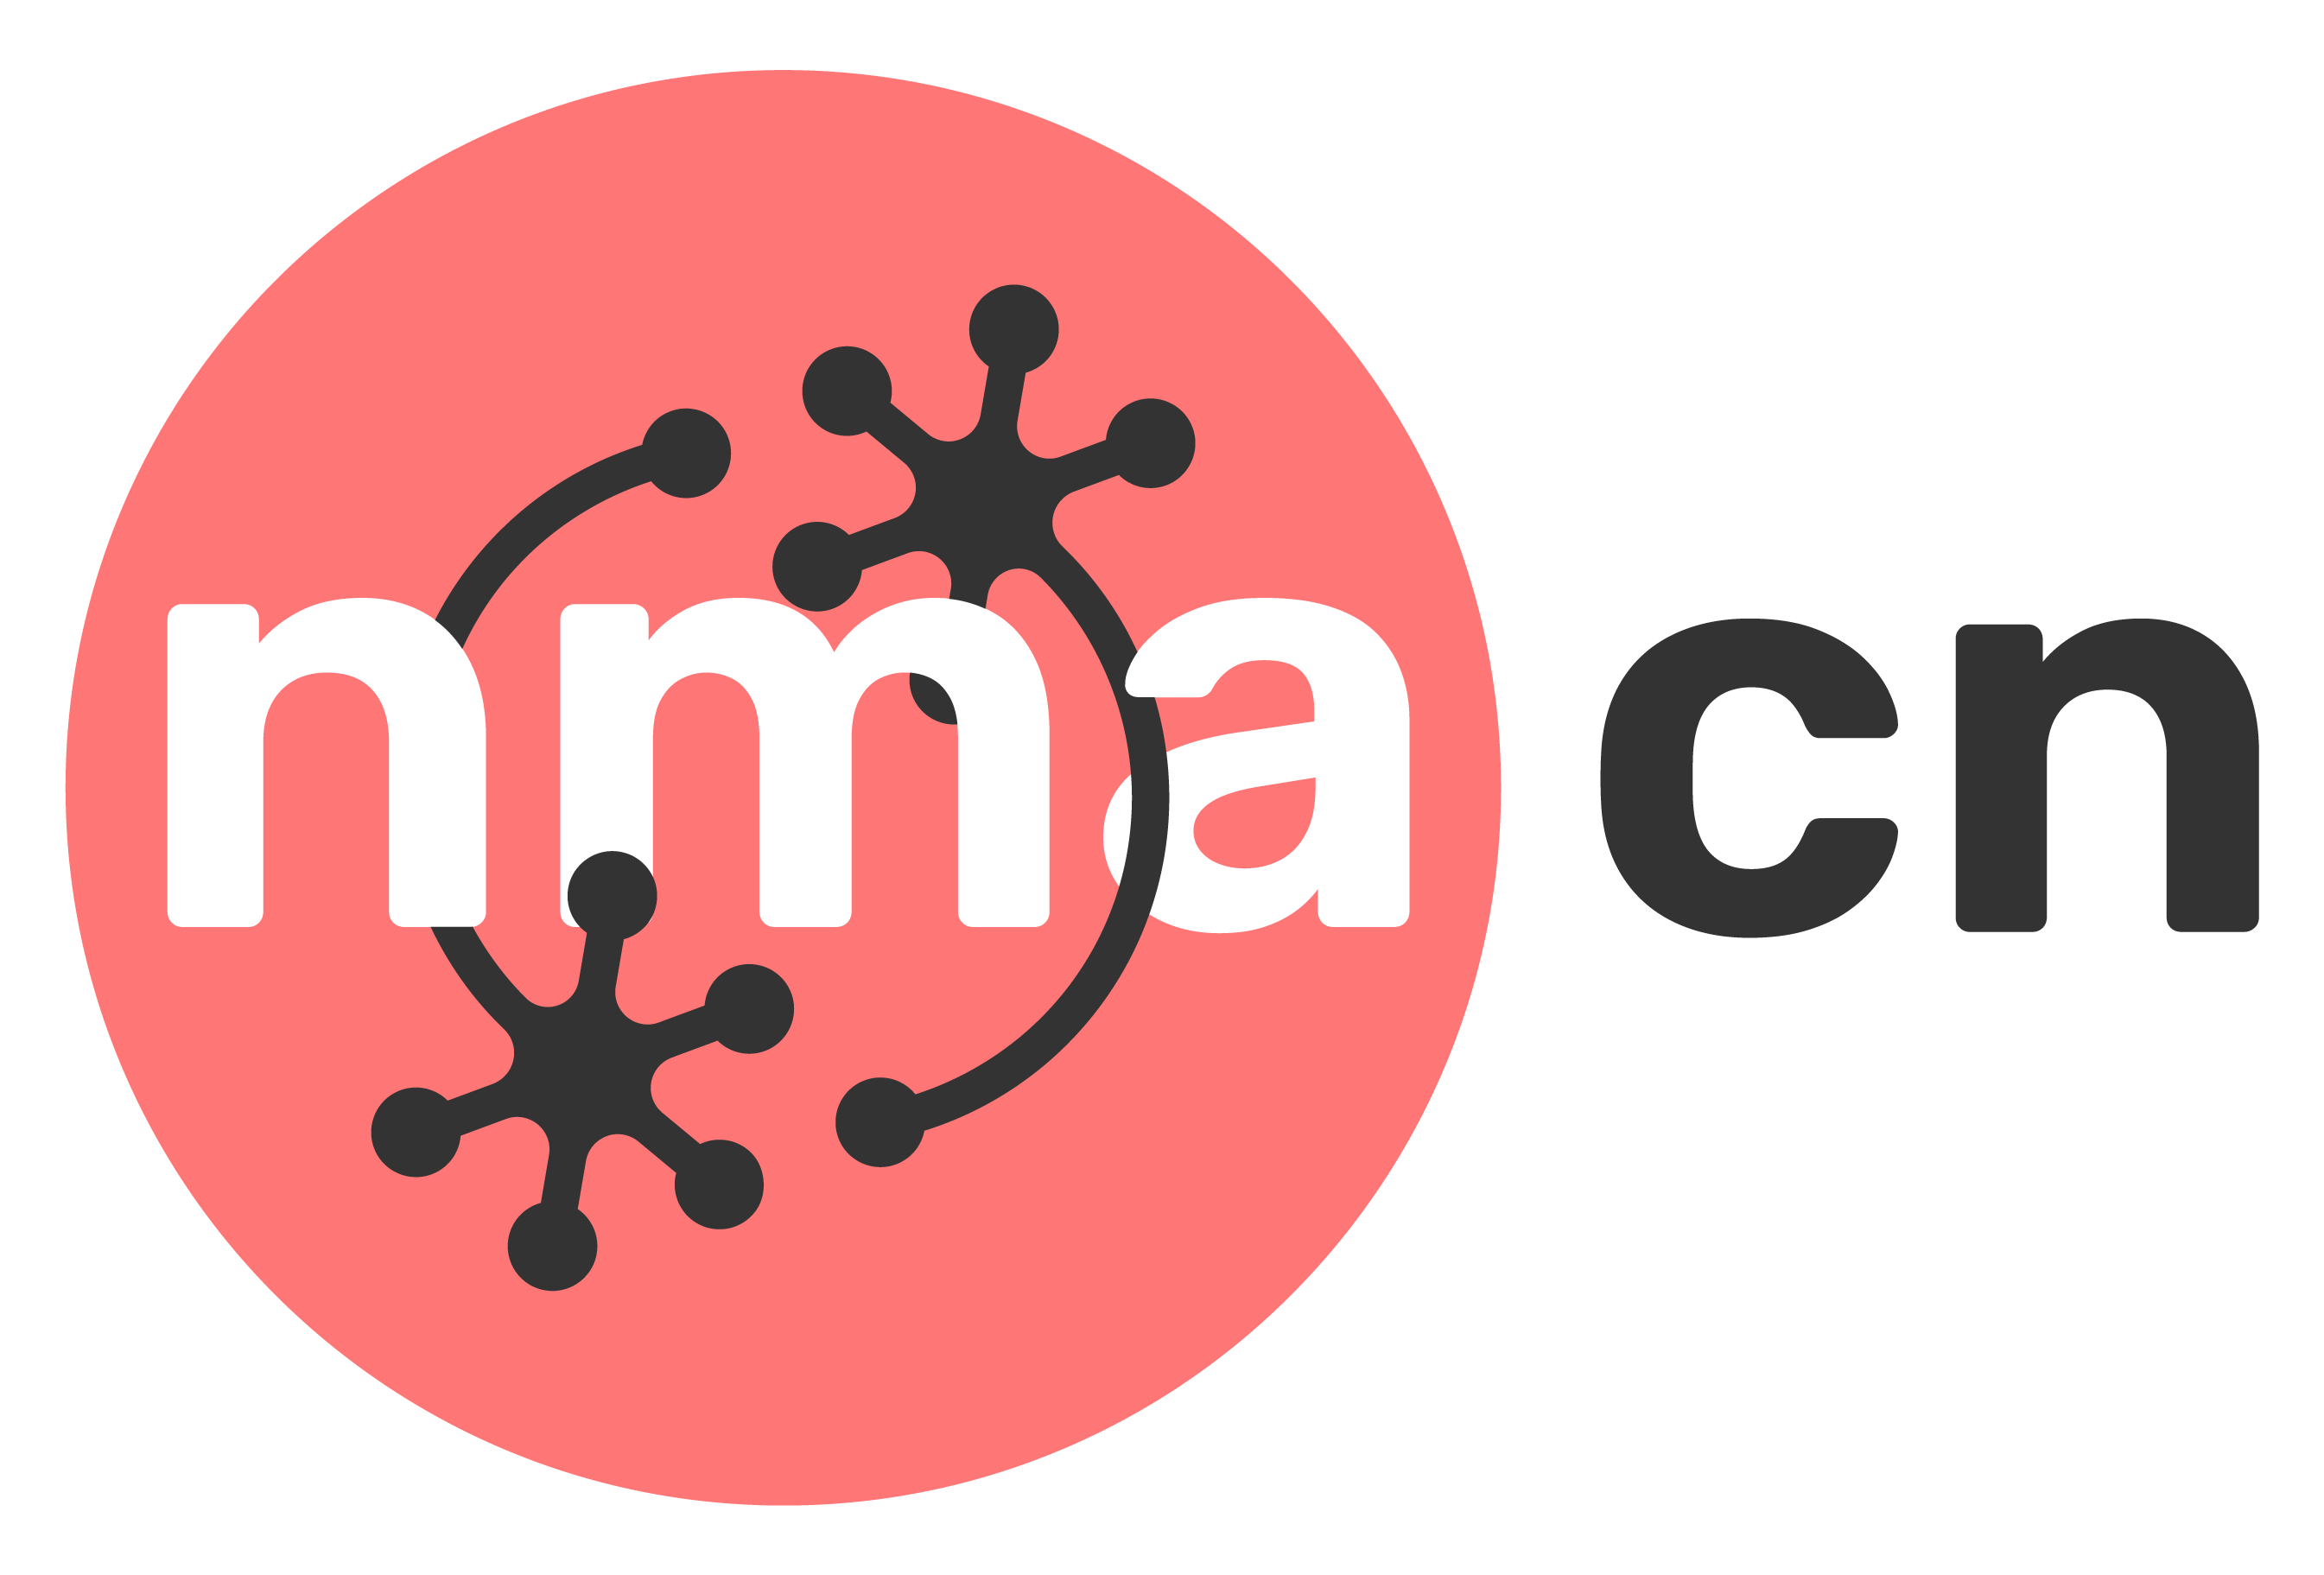
\includegraphics[scale=0.03]{Figures/NMACN.png}\href{https://compneuro.neuromatch.io/tutorials/intro.html}{\textbf{\Huge{Neuromatch Academy Model Types - Summary Sheet}}\footnote{’t Hart et al., (2022). Neuromatch Academy: a 3-week, online summer school in computational neuroscience. Journal of Open Source Education, 5(49), 118. https://doi.org/10.21105/jose.00118}}
%$\subsection*{Cheat Sheet}
\small
\begin{multicols}{3}
%\scriptsize
%\pagecolor{black}

\let\clearpage\relax
\begin{textbox}{\href{https://compneuro.neuromatch.io/tutorials/W1D1_ModelTypes/student/W1D1_Tutorial1.html}{"What" models } }
\begin{subbox}{subbox}{Overview}
\scriptsize
We will explore \textbf{"What"} models, used to describe the data. To understand what our data looks like, we will visualize it in different ways. Then we will compare it to simple mathematical models. Specifically, we will:
\begin{itemize}
    \item 
Use spiking activity from hundreds of neurons and understand how it is organized
\item Visualize characteristics of the spiking activity across the population
\item Compute the distribution of "inter-spike intervals" (ISIs) for a single neuron
\item Consider several formal models of this distribution's shape and fit them to the data "by hand"
\end{itemize}

\end{subbox}

\begin{subbox}{subbox}{Exploring the Steinmetz dataset}
\scriptsize

We consider a subset of data from a study of \href{https://www.nature.com/articles/s41586-019-1787-x}{Steinmetz et al. (2019)}. In this study, Neuropixels probes were implanted in the brains of mice. Electrical potentials were measured by hundreds of electrodes along the length of each probe. Each electrode's measurements captured local variations in the electric field due to nearby spiking neurons. A spike sorting algorithm was used to infer spike times and cluster spikes according to common origin: a single cluster of sorted spikes is causally attributed to a single neuron.

In particular, a single recording session of spike times and neuron assignments was loaded and assigned to \textit{spike times} in the preceding setup.
Typically a dataset comes with some information about its structure. However, this information may be incomplete.

You might also apply some transformations or "pre-processing" to create a working representation of the data of interest, which might go partly undocumented depending on the circumstances. In any case it is important to be able to use the available tools to investigate unfamiliar aspects of a data structure.

\end{subbox}




\end{textbox}
%%%%%%%%%%%%%%%%%%%%%%%%%%%%%%%%%%%%%%%%%%%%%%%%%%
%%%%%%%%%%%%%%%%%%%%%%%%%%%%%%%%%%%%%%%%%%%%%%%%%%
\begin{textbox}{\href{https://compneuro.neuromatch.io/tutorials/W1D1_ModelTypes/student/W1D1_Tutorial1.html}{"What" models } }
\begin{subbox}{subbox}{Plotting total spike counts}
\scriptsize

The number of spikes over the entire recording is variable between neurons. More generally, some neurons tend to spike more than others in a given period. Let's explore what the distribution of spiking looks like across all the neurons in the dataset.

The plot shows that the majority of neurons are relatively "quiet" compared to the mean, while a small number of neurons are exceptionally "loud": they must have spiked more often to reach a large count.
If the mean neuron is more active than 68\% of the population, what does that imply about the relationship between the mean neuron and the median (50th percentile) neuron?

\centering
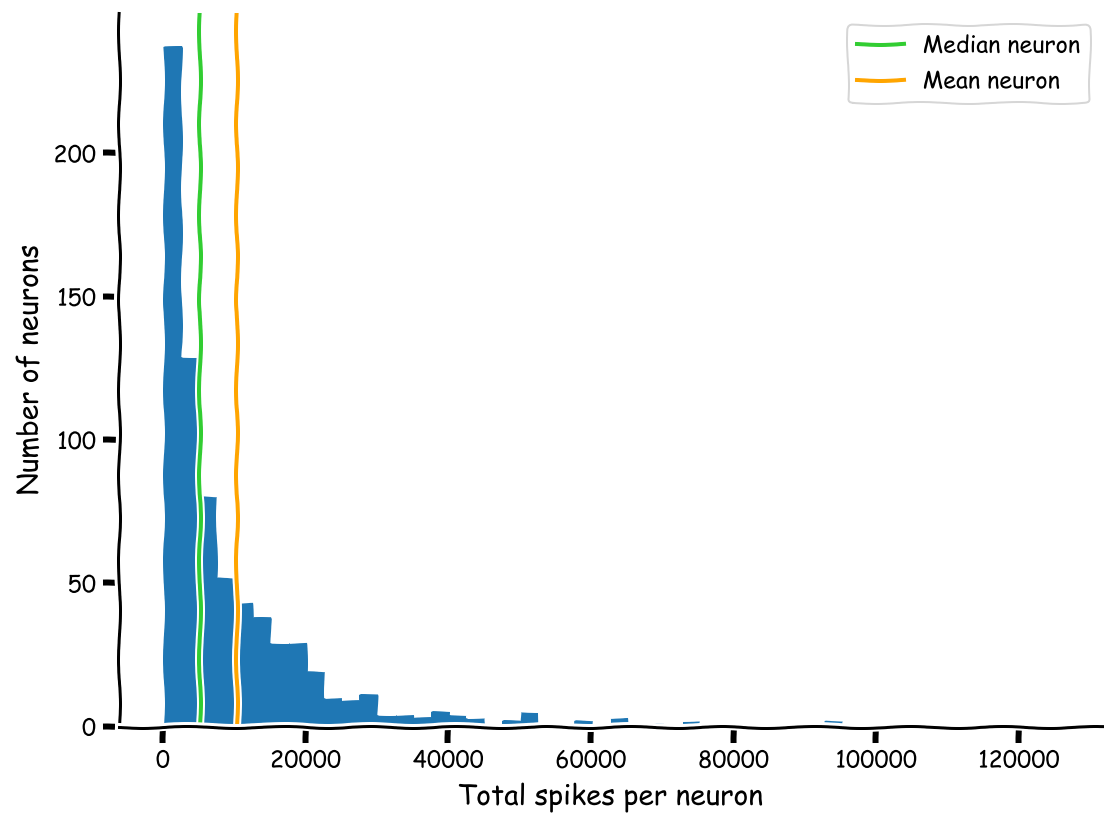
\includegraphics[scale=0.11]{Figures/MT/MT_Figure1.png}
\end{subbox}


\begin{subbox}{subbox}{Visualizing neuronal spiking activity}
\scriptsize

A "raster" plot, where the spikes from each neuron appear in a different row.

Plotting a large number of neurons can give you a sense for the characteristics in the population. 

\centering
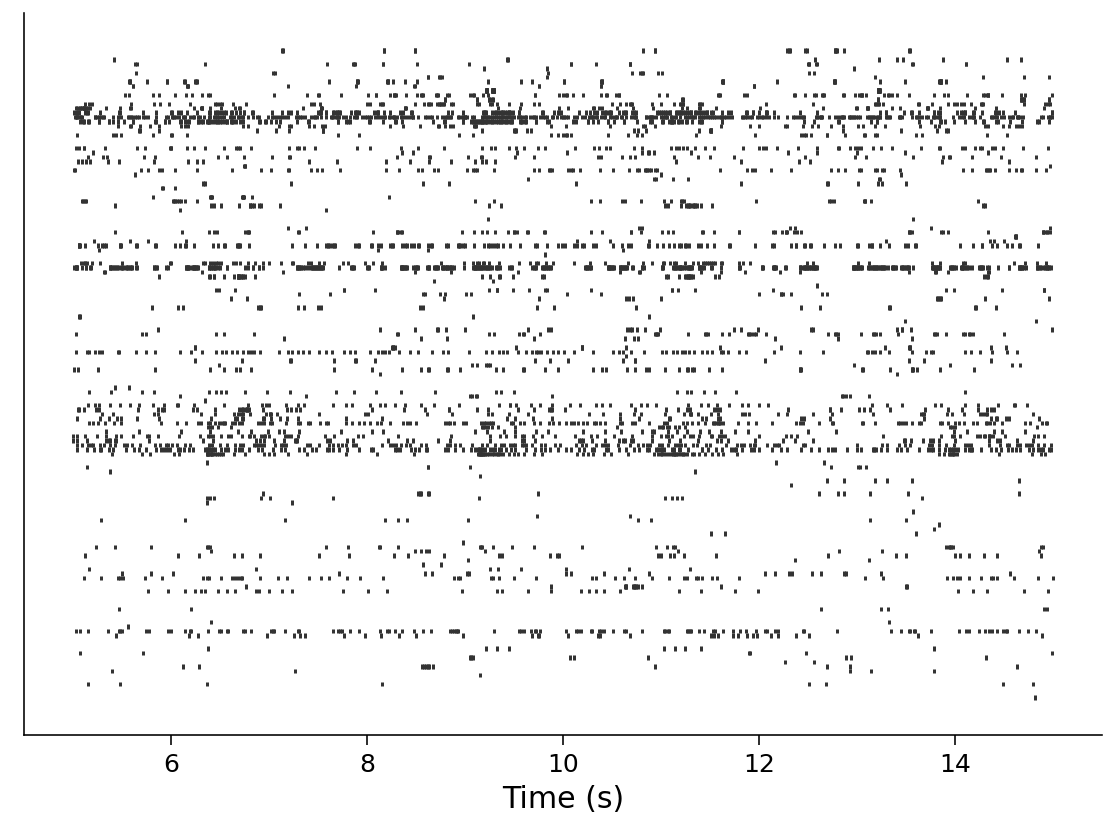
\includegraphics[scale=0.3]{Figures/MT/MT_Figure2.png}
\end{subbox}
\end{textbox}
%%%%%%%%%%%%%%%%%%%%%%%%%%%%%%%%%%%%%%%%%%%%%%%%%%
%%%%%%%%%%%%%%%%%%%%%%%%%%%%%%%%%%%%%%%%%%%%%%%%%%
\begin{textbox}{\href{https://compneuro.neuromatch.io/tutorials/W1D1_ModelTypes/student/W1D1_Tutorial1.html}{"What" models }   }
\begin{subbox}{subbox}{Inter-spike intervals and their distributions}
\scriptsize

Given the ordered arrays of spike times, what can we ask next?

Scientific questions are informed by existing models. So, what knowledge do we already have that can inform questions about this data?

We know that there are physical constraints on neuron spiking. Spiking costs energy, which the neuron's cellular machinery can only obtain at a finite rate. Therefore neurons should have a refractory period: they can only fire as quickly as their metabolic processes can support, and there is a minimum delay between consecutive spikes of the same neuron.
More generally, we can ask "how long does a neuron wait to spike again?" or "what is the longest a neuron will wait?" Can we transform spike times into something else, to address questions like these more directly?
We can consider the inter-spike times (or interspike intervals: ISIs). These are simply the time differences between consecutive spikes of the same neuron.
In general, the shorter ISIs are predominant, with counts decreasing rapidly (and smoothly, more or less) with increasing ISI. However, counts also rapidly decrease to zero with decreasing ISI below the maximum of the distribution (8-11 ms). The absence of these very low ISIs agrees with the refractory period hypothesis: the neuron cannot fire quickly enough to populate this region of the ISI distribution.

\end{subbox}
\begin{subbox}{subbox}{What is the functional form of an ISI distribution?}
\scriptsize


The ISI histograms seem to follow continuous, monotonically decreasing functions above their maxima. The function is clearly non-linear. Could it belong to a single family of functions?

To motivate the idea of using a mathematical function to explain physiological phenomena, let's define a few different function forms that we might expect the relationship to follow: exponential, inverse, and linear.

\begin{center}
    
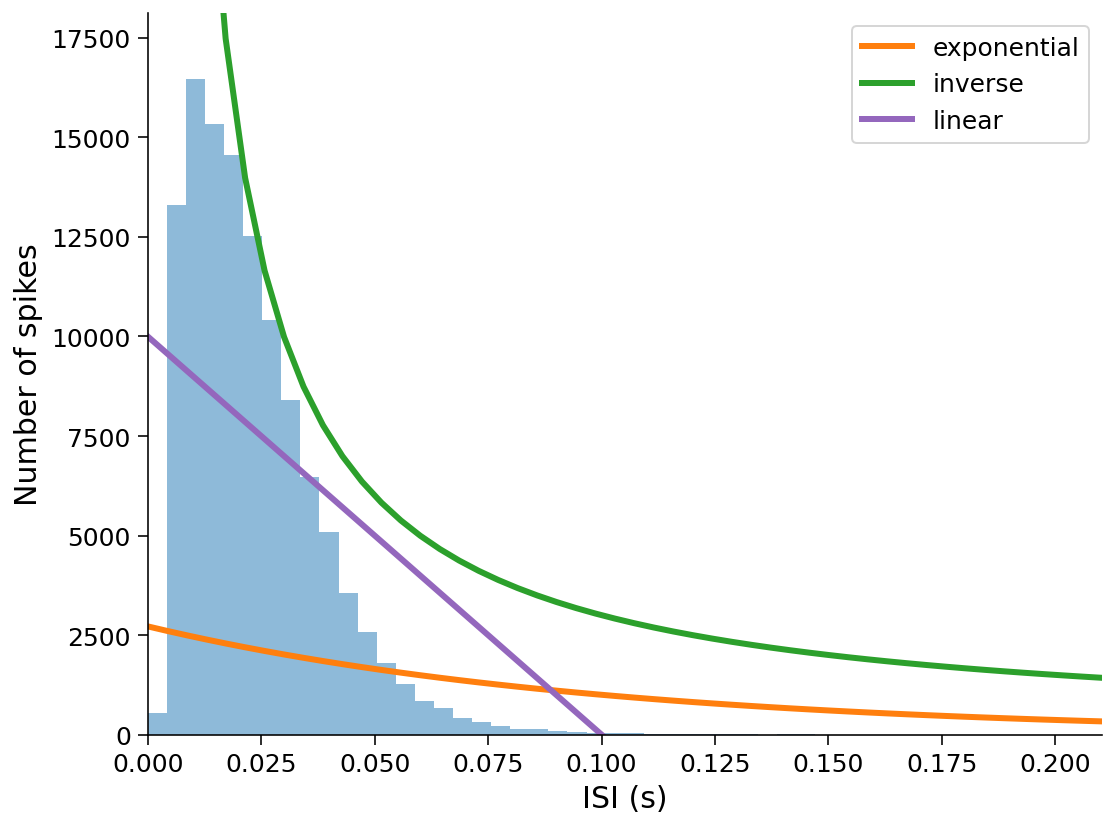
\includegraphics[scale=0.15]{Figures/MT/MT_Figure4.png}
\end{center}
The exponential function can be made to fit the data much better than the linear
or inverse function.
\end{subbox}
\end{textbox}
%%%%%%%%%%%%%%%%%%%%%%%%%%%%%%%%%%%%%%%%%%%%%%%%%%
%%%%%%%%%%%%%%%%%%%%%%%%%%%%%%%%%%%%%%%%%%%%%%%%%%
%%%TUTORIAL 2
%%%%%%%%%%%%%%%%%%%%%%%%%%%%%%%%%%%%%%%%%%%%%%%%%%
%%%%%%%%%%%%%%%%%%%%%%%%%%%%%%%%%%%%%%%%%%%%%%%%%%
\begin{textbox}{\href{https://compneuro.neuromatch.io/tutorials/W1D1_ModelTypes/student/W1D1_Tutorial2.html}{"How" models } }
\begin{subbox}{subbox}{Overview }
\scriptsize
We will explore models that can potentially explain \textbf{"How"} the spiking data we have observed is produced. To understand the mechanisms  we will build simple neuronal models and compare their spiking response to real data. We will:
\begin{enumerate}
    \item 
 Simulate a  simple "leaky integrate-and-fire" neuron model 
\item Make the model more complicated — but also more realistic—by adding more physiologically-inspired details
\end{enumerate}
\end{subbox}
\begin{subbox}{subbox}{How does a neuron spike? }
\scriptsize

A neuron charges and discharges an electric field across its cell membrane. The state of this electric field can be described by the \textit{membrane potential}. The membrane potential rises due to excitation of the neuron, and when it reaches a threshold a spike occurs. The potential resets, and must rise to a threshold again before the next spike occurs.

One of the simplest models of spiking neuron behavior is the linear integrate-and-fire (LIF) model neuron. In this model, the neuron increases its membrane potential $V_m$ over time in response to excitatory input currents $I$ scaled by some factor $\alpha$:
\begin{equation}
dV_m = {\alpha}I
\end{equation}
Once $V_m$ reaches a threshold value a spike is produced, $V_m$ is reset to a starting value, and the process continues. 

Here, we will take the starting and threshold potentials as $0$ and $1$, respectively. So, for example, if $\alpha I=0.1$ is constant---that is, the input current is constant---then $dV_m=0.1$, and at each timestep the membrane potential $V_m$ increases by $0.1$ until after $(1-0)/0.1 = 10$ timesteps it reaches the threshold and resets to $V_m=0$, and so on.

Note that we define the membrane potential $V_m$ as a scalar: a single real (or floating point) number. However, a biological neuron's membrane potential will not be exactly constant at all points on its cell membrane at a given time. We could capture this variation with a more complex model (e.g. with more numbers). Do we need to? 

The proposed model is a 1D simplification. There are many details we could add to it, to preserve different parts of the complex structure and dynamics of a real neuron. If we were interested in small or local changes in the membrane potential, our 1D simplification could be a problem. However, we'll assume an idealized "point" neuron model for our current purpose.
\begin{center}
    
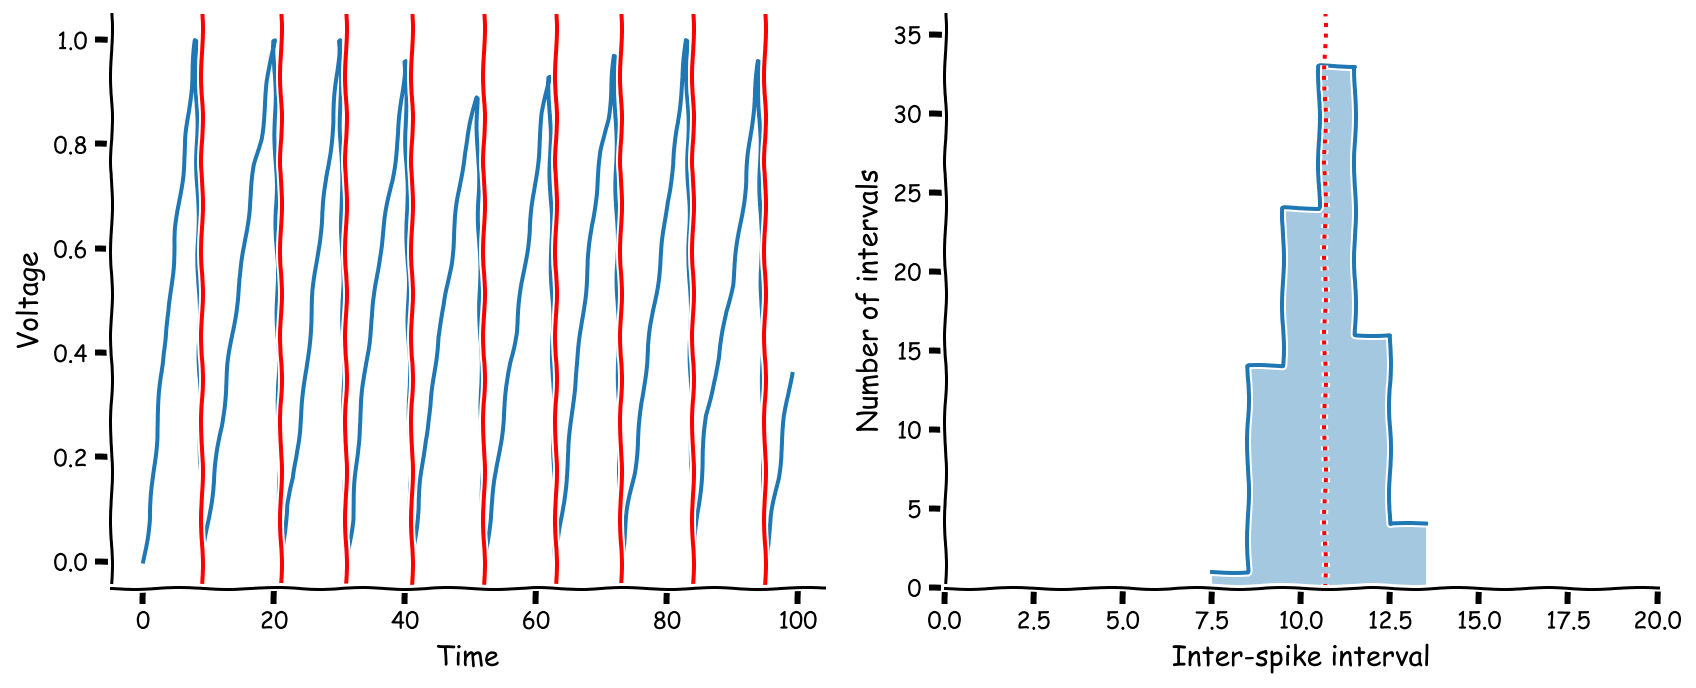
\includegraphics[scale=0.08]{Figures/MT/MT_Figure5.png}
\end{center}
\end{subbox}
\end{textbox}
%%%%%%%%%%%%%%%%%%%%%%%%%%%%%%%%%%%%%%%%%%%%%%%%%%
%%%%%%%%%%%%%%%%%%%%%%%%%%%%%%%%%%%%%%%%%%%%%%%%%%
\begin{textbox}{\href{https://compneuro.neuromatch.io/tutorials/W1D1_ModelTypes/student/W1D1_Tutorial2.html}{"How" models } }

\begin{subbox}{subbox}{Spiking Inputs}
\scriptsize

Given our simplified model for the neuron dynamics, we still need to consider what form the input $I$ will take. How should we specify the firing behavior of the presynaptic neuron(s) providing the inputs to our model neuron? 

Unlike in the simple example the input current is generally not constant. Physical inputs tend to vary with time. We can describe this variation with a distribution.

We'll assume the input current $I$ over a timestep is due to equal contributions from a non-negative ($\ge 0$) integer number of input spikes arriving in that timestep. Our model neuron might integrate currents from 3 input spikes in one timestep, and 7 spikes in the next timestep. We should see similar behavior when sampling from our distribution.

Given no other information about the input neurons, we will also assume that the distribution has a mean, and that the spiking events of the input neuron(s) are independent in time. Are these reasonable assumptions in the context of real neurons?

A suitable distribution given these assumptions is the Poisson distribution, which we'll use to model $I$:

\begin{equation}
I \sim \mathrm{Poisson}(\lambda)
\end{equation}

where $\lambda$ is the mean of the distribution: the average rate of spikes received per timestep.

\end{subbox}
\begin{subbox}{subbox}{Inhibitory signals}
\scriptsize

Our linear IF neuron from the previous section was indeed able to produce spikes. However, our ISI histogram doesn't look much like an empirical ISI histograms, which has an exponential-like shape. What is our model neuron missing, given that it doesn't behave like a real neuron?

In the previous model we only considered excitatory behavior. We know, however, that there are other factors that can drive $V_m$ down. First is the natural tendency of the neuron to return to some steady state or resting potential. We can update our previous model as follows:

\begin{equation}
dV_m = -{\beta}V_m + {\alpha}I
\end{equation}

where $V_m$ is the current membrane potential and $\beta$ is some leakage factor. This is a basic form of the popular LIF model.

We also know that in addition to excitatory presynaptic neurons, we can have inhibitory presynaptic neurons as well. We can model these inhibitory neurons with another Poisson random variable:
\begin{align}
I &= I_{\mathrm{exc}} - I_{\mathrm{inh}} \\
I_{\mathrm{exc}} &\sim \mathrm{Poisson}(\lambda_{\mathrm{exc}}) \\
I_{\mathrm{inh}} &\sim \mathrm{Poisson}(\lambda_{\mathrm{inh}})
\end{align}

where $\lambda_{\mathrm{exc}}$ and $\lambda_{\mathrm{inh}}$ are the average spike rates (per timestep) of the excitatory and inhibitory presynaptic neurons, respectively.

\end{subbox}
\end{textbox}
%%%%%%%%%%%%%%%%%%%%%%%%%%%%%%%%%%%%%%%%%%%%%%%%%%
%%%%%%%%%%%%%%%%%%%%%%%%%%%%%%%%%%%%%%%%%%%%%%%%%%
\begin{textbox}{\href{https://compneuro.neuromatch.io/tutorials/W1D1_ModelTypes/student/W1D1_Tutorial2.html}{"How" models } }

\begin{subbox}{subbox}{LIF + inhibition neuron}
\scriptsize

\begin{enumerate}
    \item 
Raising the excitatory rate while keeping inhibitory rate the same results in
more frequent firing and shorter ISIs. This makes intuitive sense - more excitatory input
means higher responses.
\item Raising the inhibitory rate while keeping the excitatory rate the same results
in less frequent firing and longer ISIs. This makes intuitive sense - more inhibitory input
means lower responses.
\item If the excitatory and inhibitory rates are equal, the average inter-spike interval
stays the same even if you raise both. This is because they balance each other out.
\item Yes, these ISIs look more exponential, like what we observed.
\end{enumerate}

\begin{center}
    
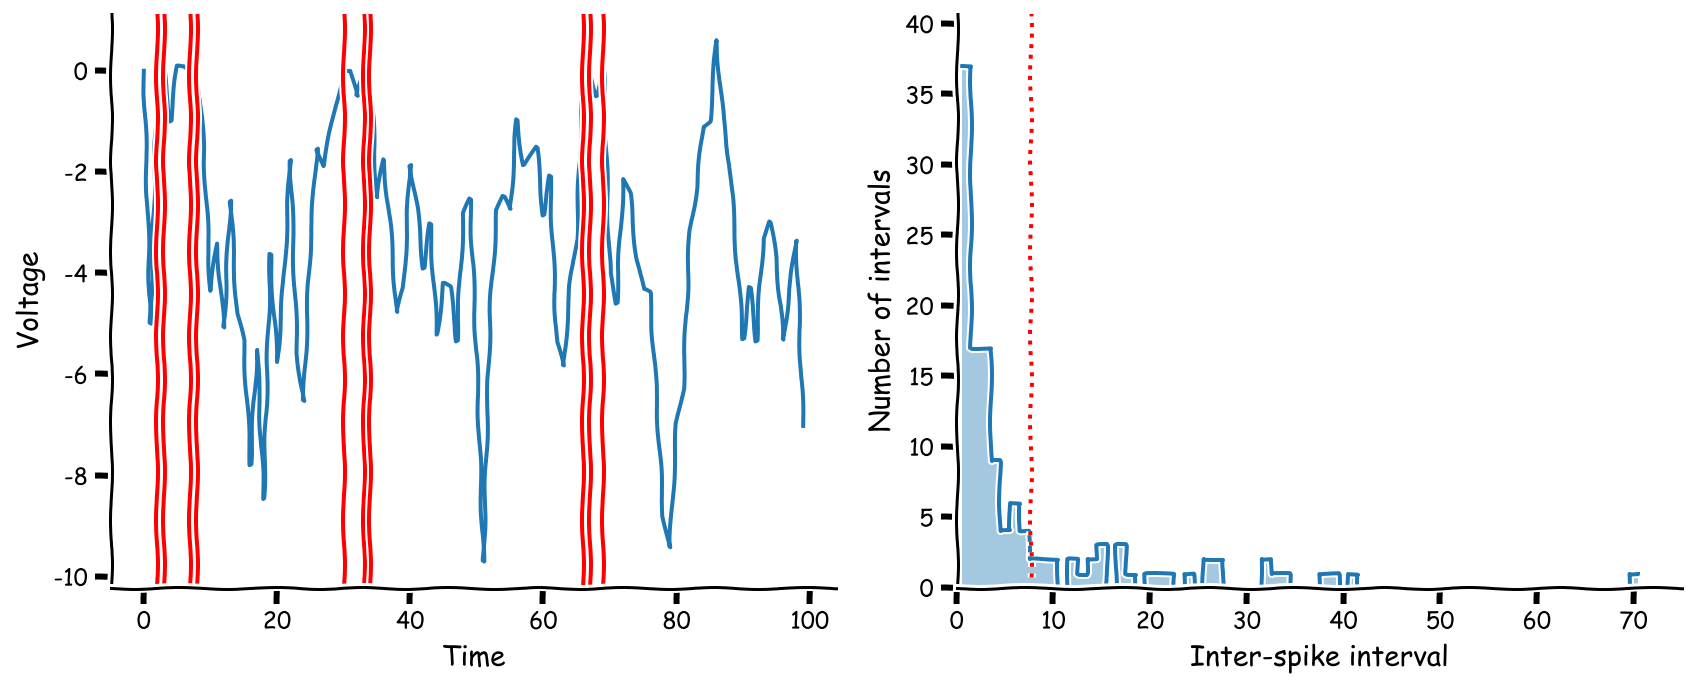
\includegraphics[scale=0.1]{Figures/MT/MT_Figure6.png}
\end{center}

\end{subbox}
\begin{subbox}{subbox}{Notation}
\scriptsize
\begin{align*}
V_m &\quad \text{membrane potential} \\
dV_m &\quad \text{change in membrane potential}\\
C_m &\quad \text{membrane capacitance}\\
I &\quad \text{input current}\\
R_m &\quad \text{membrane resistance}:\\
V_\mathrm{rest} &\quad \text{resting potential}\\
\alpha &\quad \text{scaling factor for input current}\\
\beta &\quad \text{leakage factor}\\
\lambda &\quad \text{average spike rate}\\
\lambda_\mathrm{exc} &\quad \text{average spike rate for excitatory neurons}\\
\lambda_\mathrm{inh} &\quad \text{average spike rate for inhibitory neurons}\\
\end{align*}
\end{subbox}
\end{textbox}
%%%%%%%%%%%%%%%%%%%%%%%%%%%%%%%%%%%%%%%%%%%%%%%%%%
%%%%%%%%%%%%%%%%%%%%%%%%%%%%%%%%%%%%%%%%%%%%%%%%%%
%%%%% TUTORIAL 3
%%%%%%%%%%%%%%%%%%%%%%%%%%%%%%%%%%%%%%%%%%%%%%%%%%
%%%%%%%%%%%%%%%%%%%%%%%%%%%%%%%%%%%%%%%%%%%%%%%%%%
\begin{textbox}{\href{https://compneuro.neuromatch.io/tutorials/W1D1_ModelTypes/student/W1D1_Tutorial3.html}{"Why" models }  }

\begin{subbox}{subbox}{Overview}
\scriptsize
We will explore models and techniques that can potentially explain \textbf{why} the spiking data we have observed is produced the way it is.

To understand why different spiking behaviors may be beneficial, we will learn about the concept of entropy. Specifically, we will:

\begin{enumerate}
    \item  Write code to compute formula for entropy, a measure of information
 \item  Compute the entropy of a number of toy distributions
 \item  Compute the entropy of spiking activity from the Steinmetz dataset

\end{enumerate}
\end{subbox}
\begin{subbox}{subbox}{Optimization and Information}
\scriptsize
Neurons can only fire so often in a fixed period of time, as the act of emitting a spike consumes energy that is depleted and must eventually be replenished. To communicate effectively for downstream computation, the neuron would need to make good use of its limited spiking capability. This becomes an optimization problem: 

What is the optimal way for a neuron to fire in order to maximize its ability to communicate information?

In order to explore this question, we first need to have a quantifiable measure for information. Shannon introduced the concept of entropy to do just that, and defined it as

\begin{equation}
H_b(X) = -\sum_{x\in X} p(x) \log_b p(x)
\end{equation}

where $H$ is entropy measured in units of base $b$ and $p(x)$ is the probability of observing the event $x$ from the set of all possible events in $X$. See the Bonus Section 1 for a more detailed look at how this equation was derived.

The most common base of measuring entropy is $b=2$, so we often talk about \textbf{bits} of information, though other bases are used as well (e.g. when $b=e$ we call the units \textit{nats}).

A distribution with mass split equally between two points looks like:

\begin{center}
    
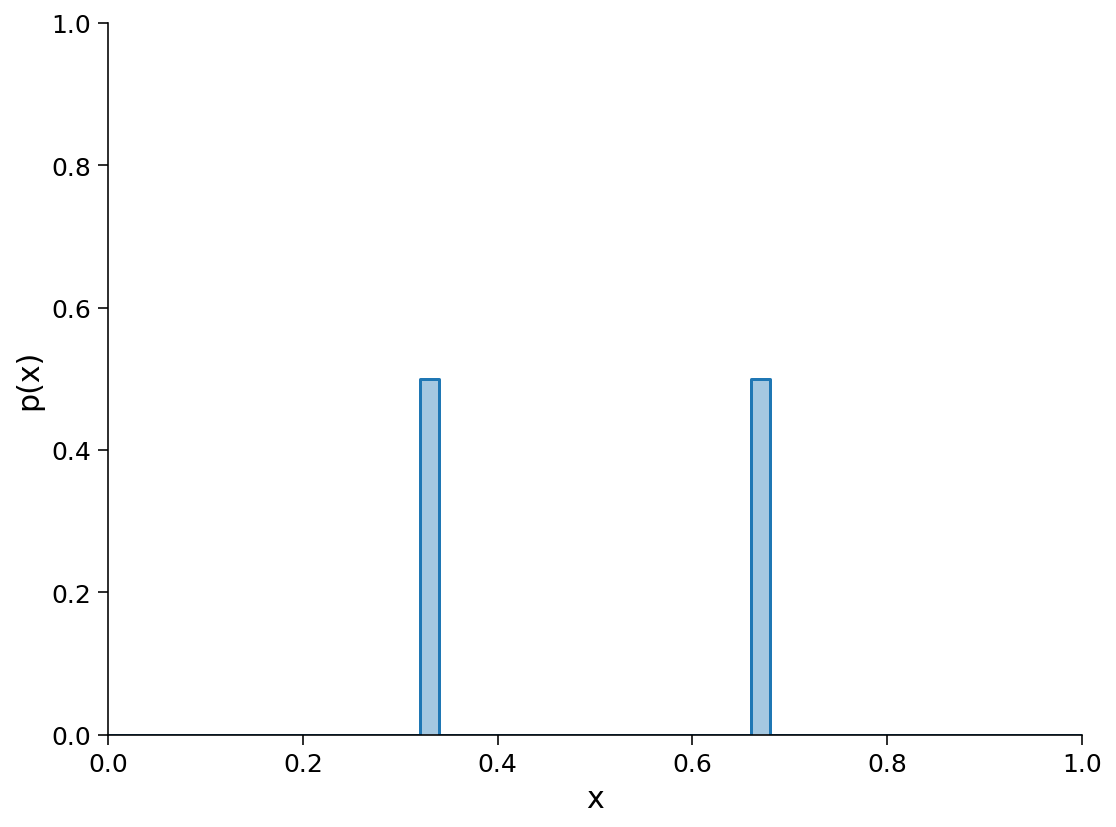
\includegraphics[scale=0.2]{Figures/MT/MT_Figure7.png}
\end{center}

Here, the entropy calculation is: $-(0.5 \log_2 0.5 + 0.5\log_2 0.5)=1$
ere is 1 bit of entropy. This means that before we take a random sample, there is 1 bit of uncertainty about which point in the distribution the sample will fall on: it will either be the first peak or the second one. 

\end{subbox}
\end{textbox}
%%%%%%%%%%%%%%%%%%%%%%%%%%%%%%%%%%%%%%%%%%%%%%%%%%
%%%%%%%%%%%%%%%%%%%%%%%%%%%%%%%%%%%%%%%%%%%%%%%%%%
\begin{textbox}{\href{https://compneuro.neuromatch.io/tutorials/W1D1_ModelTypes/student/W1D1_Tutorial3.html}{"Why" models } }


\begin{subbox}{subbox}{Entropy}
\scriptsize


Likewise, if we make one of the peaks taller and the other one shorter, the entropy will decrease because of the increased certainty that the sample will fall on one point and not the other: : $-(0.2 \log_2 0.2 + 0.8\log_2 0.8)\approx 0.72$

If we split the probability mass among even more points, the entropy continues to increase. Let's derive the general form for $N$ points of equal mass, where $p_i=p=1/N$:

\begin{align}
-\sum_i p_i \log_b p_i &= -\sum_i^N \frac{1}{N} \log_b \frac{1}{N} \\
&= -\log_b \frac{1}{N} \\
&= \log_b N
\end{align}

If we have $N$ discrete points, the \textit{uniform distribution} (where all points have equal mass) is the distribution with the highest entropy: $\log_b N$. This upper bound on entropy is useful when considering binning strategies, as any estimate of entropy over $N$ discrete points (or bins) must be in the interval $[0, \log_b N]$

\end{subbox}

\begin{subbox}{subbox}{Information, neurons, and spikes}
\scriptsize
We'll consider three hypothetical neurons that all have the same mean ISI, but with different distributions:
\begin{enumerate}
\item Deterministic
\item Uniform
\item Exponential
\end{enumerate}
Fixing the mean of the ISI distribution is equivalent to fixing its inverse: the neuron's mean firing rate. If a neuron has a fixed energy budget and each of its spikes has the same energy cost, then by fixing the mean firing rate, we are normalizing for energy expenditure. This provides a basis for comparing the entropy of different ISI distributions. In other words: if our neuron has a fixed budget, what ISI distribution should it express (all else being equal) to maximize the information content of its outputs?

Let's construct our three distributions and see how their entropies differ.

\begin{center}
    
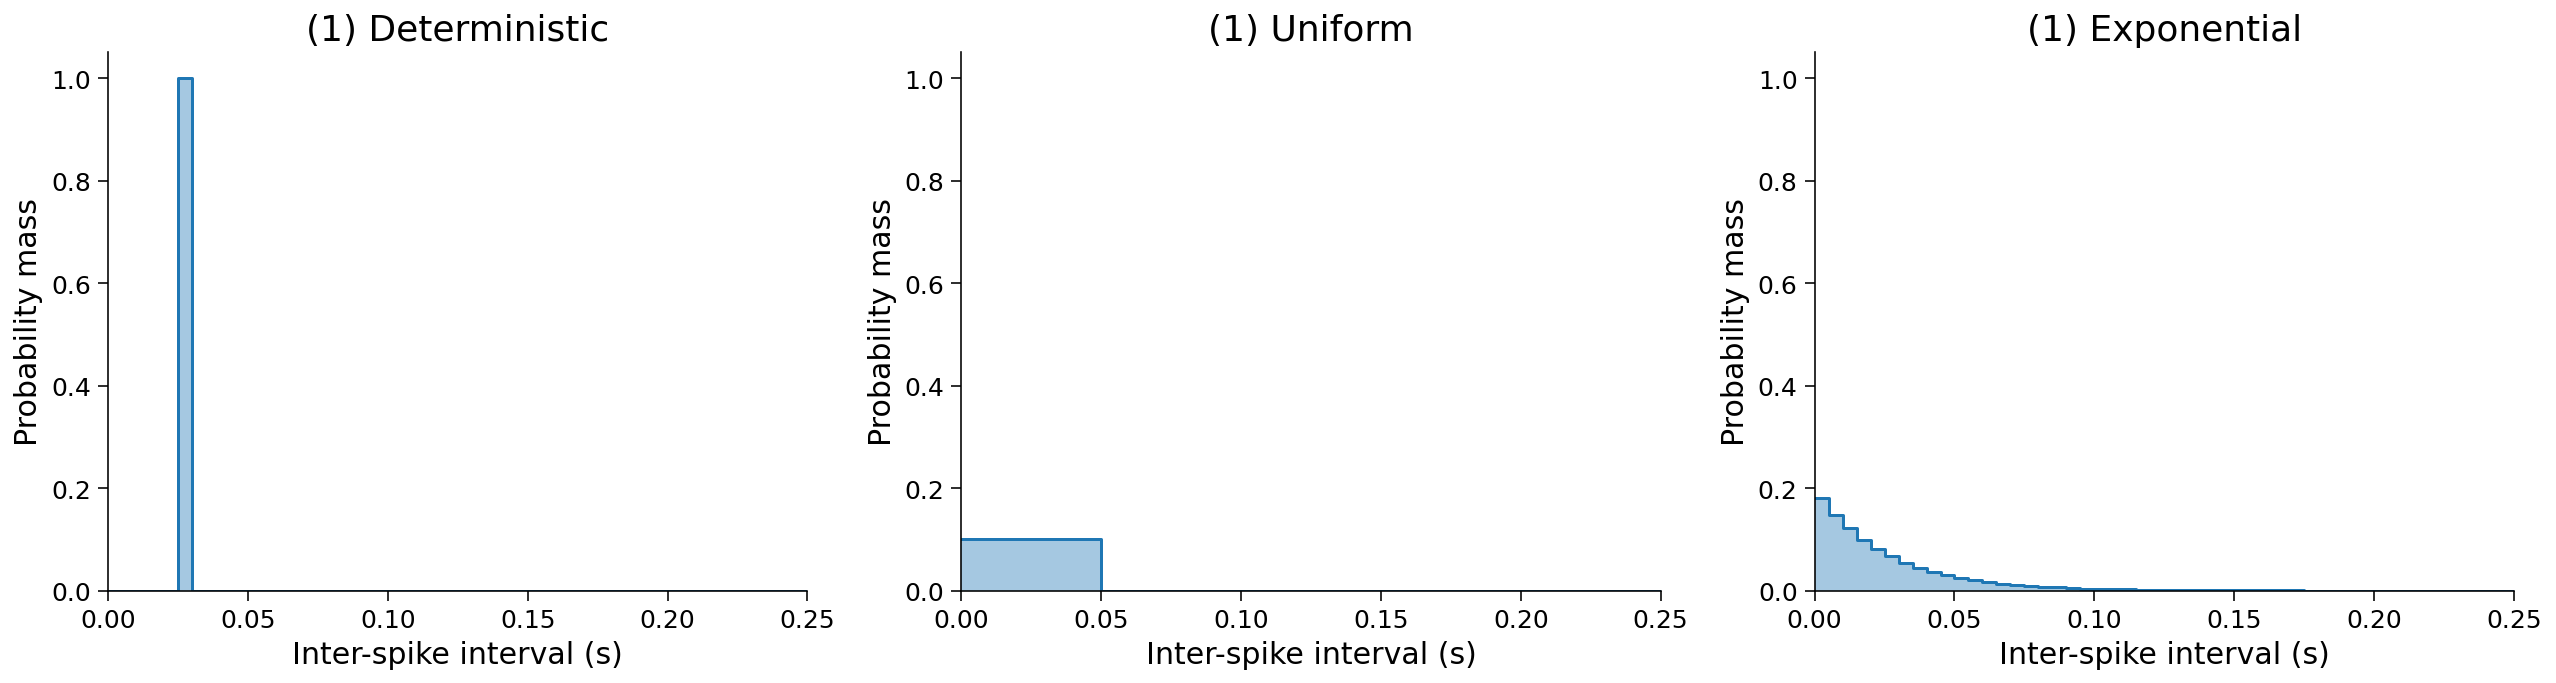
\includegraphics[scale=0.14]{Figures/MT/MT_Figure8.png}
\end{center}


\begin{enumerate}
\item Deterministic: 0.00 bits
\item Uniform: 3.32 bits
\item Exponential: 3.77 bits
\end{enumerate}
\end{subbox}

\end{textbox}
%%%%%%%%%%%%%%%%%%%%%%%%%%%%%%%%%%%%%%%%%%%%%%%%%%
%%%%%%%%%%%%%%%%%%%%%%%%%%%%%%%%%%%%%%%%%%%%%%%%%%
\begin{textbox}{\href{https://compneuro.neuromatch.io/tutorials/W1D1_ModelTypes/student/W1D1_Tutorial3.html}{"Why" models } }


\begin{subbox}{subbox}{Calculate entropy of ISI distributions from data
}
\scriptsize


In the previous example we created the PMFs by hand to illustrate idealized scenarios. How would we compute them from data recorded from actual neurons?

One way is to convert the ISI histograms we've previously computed into discrete probability distributions using the following equation:

\begin{equation}
p_i = \frac{n_i}{\sum\nolimits_{i}n_i}
\end{equation}

where $p_i$ is the probability of an ISI falling within a particular interval $i$ and $n_i$ is the count of how many ISIs were observed in that interval.

\begin{center}
    
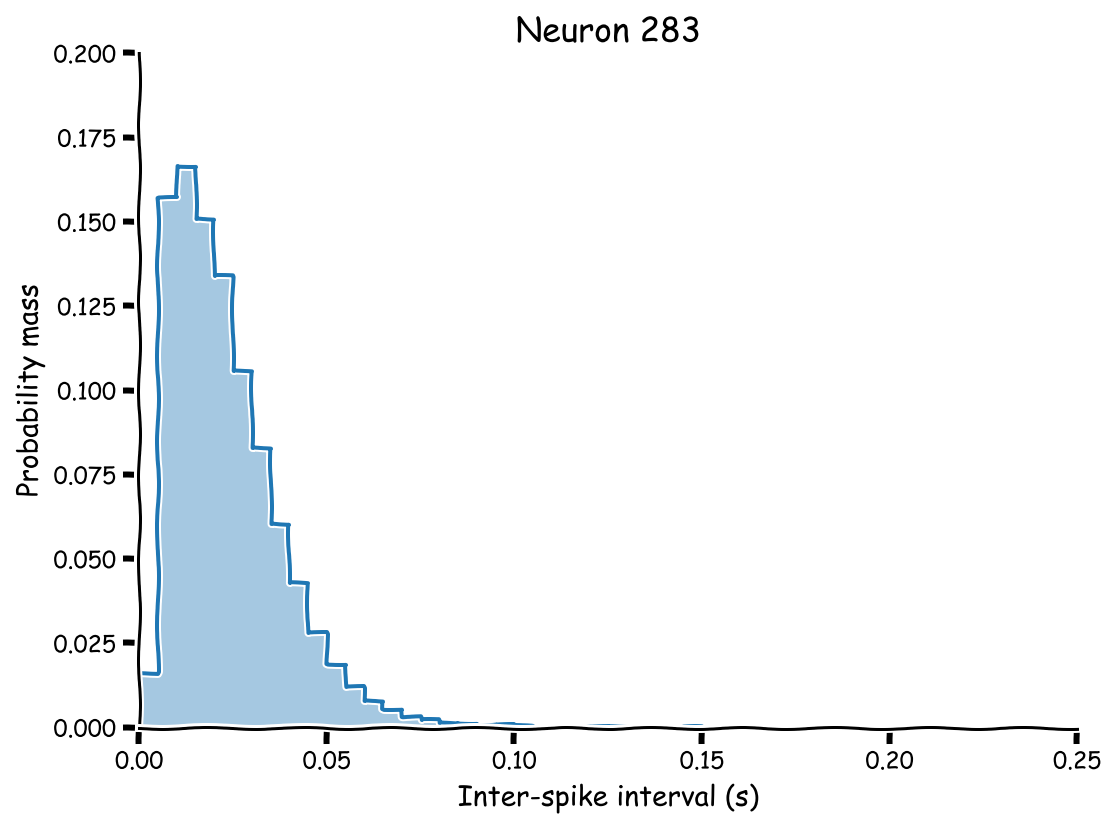
\includegraphics[scale=0.1]{Figures/MT/MT_Figure9.png}
\end{center}
Entropy for Neuron 283: 3.36 bits

\end{subbox}

\begin{subbox}{subbox}{Summary}
\scriptsize
We used different types of models to understand the spiking behavior of neurons recorded in the Steinmetz data set. 

\begin{itemize}
\item We used "what" models to discover that the ISI distribution of real neurons is closest to an exponential distribution
\item We used "how" models to discover that balanced excitatory and inhibitory inputs, coupled with a leaky membrane, can give rise to neuronal spiking with exhibiting such an exponential ISI distribution
 \item We used "why" models to discover that exponential ISI distributions contain the most information when the mean spiking is constrained
\end{itemize}
\end{subbox}

\begin{subbox}{subbox}{Notation}
\tiny
\begin{align*}
H(X) &\quad \text{entropy of random variable X}\\
b &\quad \text{base, e.g. b=2 or b=e}\\
x &\quad \text{event x}\\
p(x) &\quad \text{probability of observing event x}\\
\text{ISI} &\quad \text{interspike interval}\\
n_i &\quad \text{count of observed ISIs in interval i}\\
p_i  &\quad \text{probability of of an ISI falling within a particular interval i}
\end{align*}
\end{subbox}
\end{textbox}

\end{multicols}

\newpage
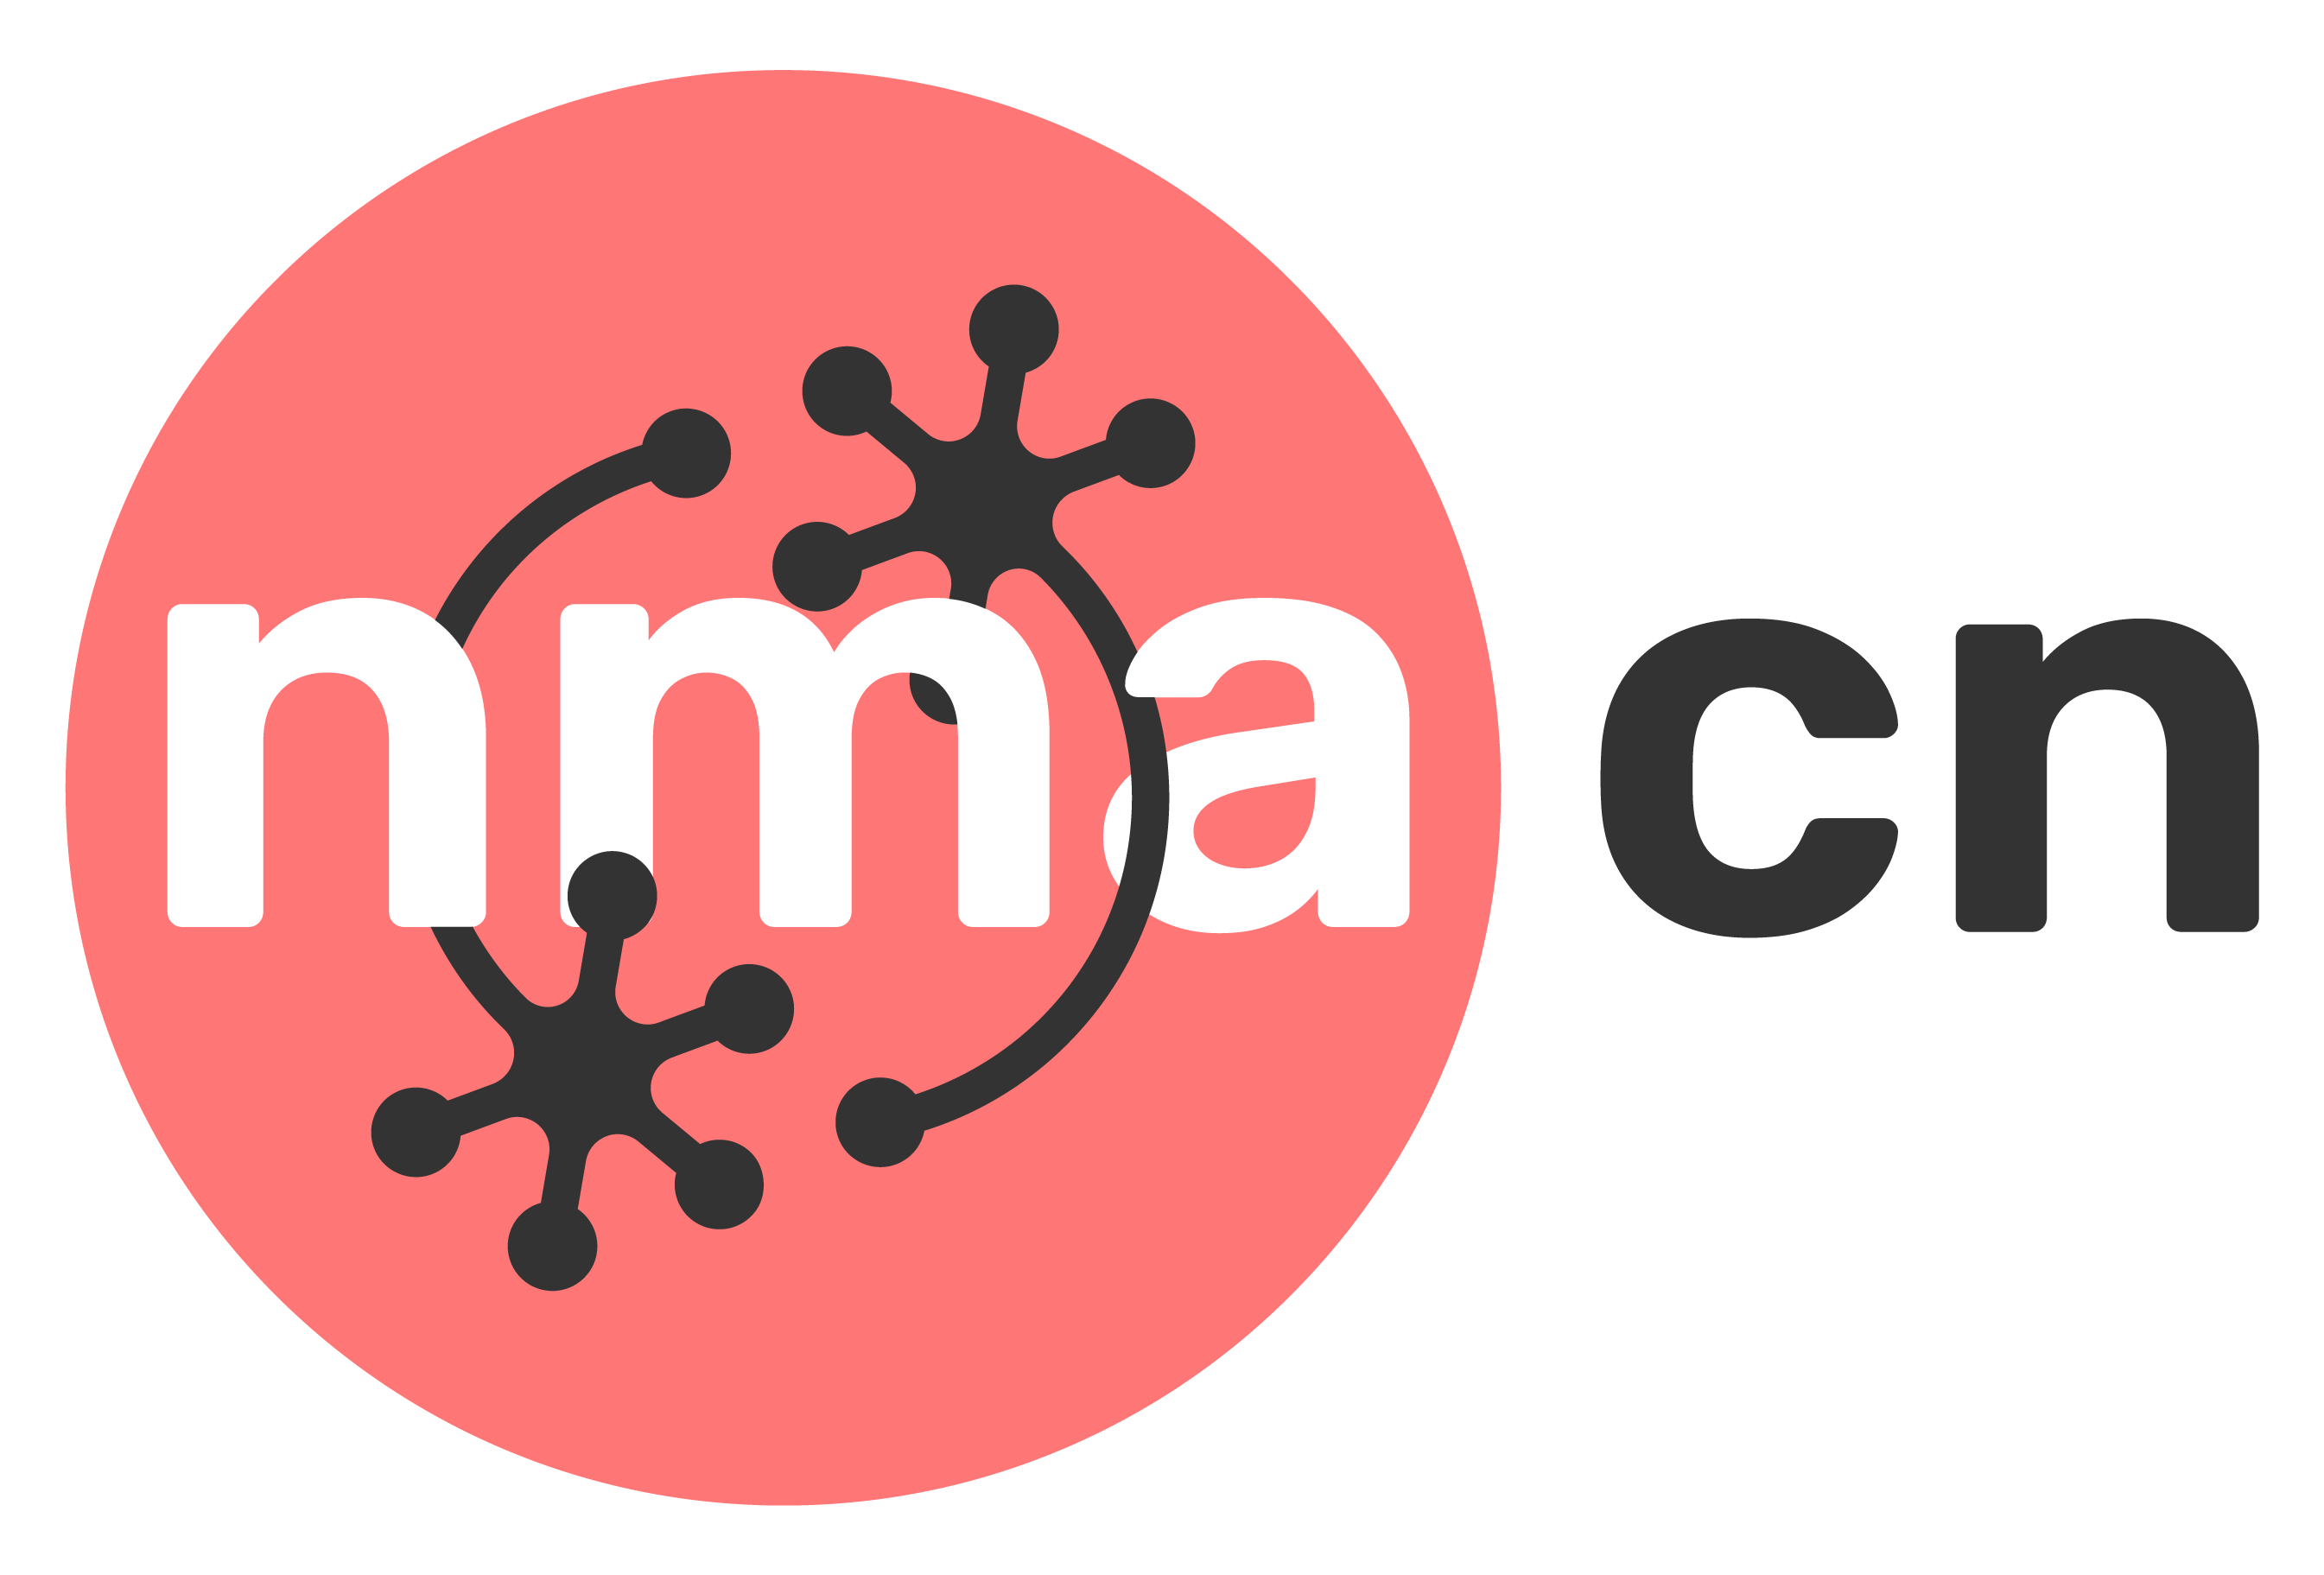
\includegraphics[scale=0.03]{Figures/NMACN.png}\href{https://compneuro.neuromatch.io/tutorials/W1D2_ModelingPractice/chapter_title.html}{\textbf{\Huge{Neuromatch Academy Modeling Practice - Summary Sheet}}\footnote{’t Hart et al., (2022). Neuromatch Academy: a 3-week, online summer school in computational neuroscience. Journal of Open Source Education, 5(49), 118. https://doi.org/10.21105/jose.00118}}
\begin{multicols}{3}
\clearpage
\begin{textbox}{\href{https://compneuro.neuromatch.io/projects/modelingsteps/ModelingSteps_5through10.html}{Modeling Practice } }
\begin{subbox}{subbox}{Framing the Question}
\scriptsize
We will try to clarify the process of computational modeling, by thinking through the logic of modeling a project.

We assume that you have a general idea of a project in mind, i.e. a preliminary question, and/or phenomenon you would like to understand. You should have started developing a project idea yesterday with \href{https://youtu.be/H6rSlZzlrgQ}{this brainstorming demo}. Maybe you have a goal in mind. We will now work through the 4 first steps of modeling (\href{https://doi.org/10.1523/ENEURO.0352-19.2019}{Blohm et al., 2019}): 

\textbf{Framing the question:}\\
\begin{enumerate}    \item 
 finding a phenomenon and a question to ask about it
    \item 
 understanding the state of the art
    \item 
 determining the basic ingredients
    \item 
 formulating specific, mathematically defined hypotheses
\end{enumerate}

The remaining steps 5-10 are covered later.

\textbf{Importantly}, we will guide you through Steps 1-4 today. After you do more work on projects, you likely have to revise some or all of these steps *before* you move on to the remaining steps of modeling.  "Models" here can be data analysis pipelines, not just computational models...

\end{subbox}
%%%%%%%%%%%%%%%%%%%%%%%%%%%%%%%%%%%%%%%%%%%%%%%%%%
%%%%%%%%%%%%%%%%%%%%%%%%%%%%%%%%%%%%%%%%%%%%%%%%%%
\end{textbox}
%%%%%%%%%%%%%%%%%%%%%%%%%%%%%%%%%%%%%%%%%%%%%%%%%%
%%%%%%%%%%%%%%%%%%%%%%%%%%%%%%%%%%%%%%%%%%%%%%%%%%
\begin{textbox}{\href{https://compneuro.neuromatch.io/projects/modelingsteps/ModelingSteps_5through10.html}{Modeling Practice } }

\begin{subbox}{subbox}{Step 1 - Asking your own question }
\scriptsize
You should already have a project idea from your brainstorming yesterday. \textbf{Write down the phenomenon, question and goal(s) if you have them.} 

As a reminder, here is what you should discuss and write down:\\
  What exact aspect of data needs modeling?
  \begin{itemize}
    \item Answer this question clearly and precisely!
Otherwise you will get lost (almost guaranteed)
  \item Write everything down!
  \item  Also identify aspects of data that you do not want to address (yet)
  \end{itemize}
  
Define an evaluation method!
  \begin{itemize}
    \item How will you know your modeling is good?
     \item E.g. comparison to specific data (quantitative method of comparison?)
    \end{itemize}
 For computational models: think of an experiment that could test your model
\begin{itemize}
    \item
   You essentially want your model to interface with this experiment, i.e. you want to simulate this experiment
  
\end{itemize}

You can find interesting questions by looking for phenomena that differ from your expectations. In \textbf{what} way does it differ? \textbf{How} could that be explained (starting to think about mechanistic questions and structural hypotheses)? \textbf{Why} could it be the way it is? What experiment could you design to investigate this phenomenon? What kind of data would you need?

\end{subbox}

\begin{subbox}{subbox}{Step 1 - Make sure to avoid the pitfalls! }
\scriptsize

Question is too general
\begin{itemize}
     \item Remember: science advances one small step at the time. Get the small step right…  \end{itemize}
 Precise aspect of phenomenon you want to model is unclear
  \begin{itemize}
     \item You will fail to ask a meaningful question<  \end{itemize}
 You have already chosen a toolkit
 \begin{itemize}
     \item This will prevent you from thinking deeply about the best way to answer your scientific question
   \end{itemize}

 You don’t have a clear goal
 \begin{itemize}
     \item What do you want to get out of modeling? \end{itemize}
 You don’t have a potential experiment in mind
 \begin{itemize}
     \item 
 This will help concretize your objectives and think through the logic behind your goal
 \end{itemize}
 
  \end{subbox}
\end{textbox}
%%%%%%%%%%%%%%%%%%%%%%%%%%%%%%%%%%%%%%%%%%%%%%%%%%
%%%%%%%%%%%%%%%%%%%%%%%%%%%%%%%%%%%%%%%%%%%%%%%%%%
\begin{textbox}{\href{https://compneuro.neuromatch.io/projects/modelingsteps/ModelingSteps_5through10.html}{Modeling Practice } }

\begin{subbox}{subbox}{Step 2 - Understanding the state of the art \& background}
\scriptsize
Here is what you should get out of it:\\
Survey the literature
\begin{itemize}
    \item 
   What’s known?
  \item  What has already been done?
  \item  Previous models as a starting point?
  \item  What hypotheses have been emitted in the field?
  \item  Are there any alternative / complementary modeling approaches?
  \end{itemize}

What skill sets are required?
\begin{itemize}

  \item  Do I need to learn something before I can start?
  \item  Ensure that no important aspect is missed
  \end{itemize}

Potentially provides specific data sets / alternative modeling approaches for comparison

\end{subbox}

\end{textbox}
%%%%%%%%%%%%%%%%%%%%%%%%%%%%%%%%%%%%%%%%%%%%%%%%%%
%%%%%%%%%%%%%%%%%%%%%%%%%%%%%%%%%%%%%%%%%%%%%%%%%%
\begin{textbox}{\href{https://compneuro.neuromatch.io/projects/modelingsteps/ModelingSteps_5through10.html}{Modeling Practice } }

\begin{subbox}{subbox}{Step 3 - Determining the basic ingredients }
\scriptsize

This will allow you to think deeper about what your modeling project will need. It's a crucial step before you can formulate hypotheses because you first need to understand what your modeling approach will need. There are 2 aspects you want to think about:



1.   What parameters / variables are needed? 
\begin{itemize}
    \item 
     Constants?
      \item Do they change over space, time, conditions…?
     \item What details can be omitted?
      \item Constraints, initial conditions?
      \item Model inputs / outputs?
      \end{itemize}  
2.   Variables needed to describe the process to be modeled?
\begin{itemize}
     \item Brainstorming!
     \item What can be observed / measured?  latent variables?    
     \item Where do these variables come from?
     \item Do any abstract concepts need to be instantiated as variables?
       \item E.g. value, utility, uncertainty, cost, salience, goals, strategy, plant, dynamics
        \item Instantiate them so that they relate to potential measurements!
\end{itemize}  
This is a step where your prior knowledge and intuition is tested. You want to end up with an inventory of \textit{specific} concepts and/or interactions that need to be instantiated. 

  \end{subbox}
\begin{subbox}{subbox}{Step 3 - Pitfalls }
\scriptsize


I’m experienced, I don’t need to think about ingredients anymore
 \begin{itemize}
    \item Or so you think… \end{itemize} 

I can’t think of any ingredients
\begin{itemize}
    \item Think about the potential experiment. What are your stimuli? What parameters? What would you control? What do you measure? \end{itemize} 

I have all inputs and outputs
 \begin{itemize}
    \item Good! But what will link them? Thinking about that will start shaping your model and hypotheses \end{itemize} 

I can’t think of any links (= mechanisms)
 \begin{itemize}
    \item You will acquire a library of potential mechanisms as you keep modeling and learning
   \item But the literature will often give you hints through hypotheses
  \item If you still can't think of links, then maybe you're missing ingredients?
 \end{itemize} 
 \end{subbox}
 
 
\end{textbox}

%%%%%%%%%%%%%%%%%%%%%%%%%%%%%%%%%%%%%%%%%%%%%%%%%%
%%%%%%%%%%%%%%%%%%%%%%%%%%%%%%%%%%%%%%%%%%%%%%%%%%

%%%%%%%%%%%%%%%%%%%%%%%%%%%%%%%%%%%%%%%%%%%%%%%%%%
%%%%%%%%%%%%%%%%%%%%%%%%%%%%%%%%%%%%%%%%%%%%%%%%%%
\begin{textbox}{\href{https://compneuro.neuromatch.io/projects/modelingsteps/ModelingSteps_5through10.html}{Modeling Practice } }

\begin{subbox}{subbox}{Step 4 - Formulating your hypothesis  }
\scriptsize

Once you have your question and goal lined up, you have done a literature review (let's assume for now) and you have thought about ingredients needed for your model, you're now ready to start thinking about \textit{specific} hypotheses.

Formulating hypotheses really consists of two consecutive steps:\\



1.   You think about the hypotheses in words by relating ingredients identified in Step 3
\begin{itemize}
    \item 
       What is the model mechanism expected to do? 
          \item  How are different parameters expected to influence model results?
      \end{itemize}

2.   You then express these hypotheses in mathematical language by giving the ingredients identified in Step 3 specific variable names. 
\begin{itemize}
         \item  Be explicit, e.g. $y(t)=f(x(t),k)$ but $z(t)$ doesn’t influence $y$
          \end{itemize}



There are also "structural hypotheses" that make assumptions on what model components you hypothesize will be crucial to capture the phenomenon at hand.\\ 

\textbf{Important}: Formulating the hypotheses is the last step before starting to model. This step determines the model approach and ingredients. It provides a more detailed description of the question / goal from Step 1. The more precise the hypotheses, the easier the model will be to justify. 
  \end{subbox}
\begin{subbox}{subbox}{Step 4 - Pitfalls }
\scriptsize

I don’t need hypotheses, I will just play around with \begin{itemize}
    \item Hypotheses help determine and specify goals. You can (and should) still play… \end{itemize}

My hypotheses don’t match my question (or vice versa)
 \begin{itemize}
    \item This is a normal part of the process!</li>
\item You need to loop back to Step 1 and revisit your question / phenomenon / goals \end{itemize}

I can’t write down a math hypothesis
\begin{itemize}
    \item Often that means you lack ingredients and/or clarity on the hypothesis
  \item OR: you have a “structural” hypothesis, i.e. you expect a certain model component to be crucial in explaining the phenomenon / answering the question \end{itemize}

 \end{subbox}
 
 
\end{textbox}

%%%%%%%%%%%%%%%%%%%%%%%%%%%%%%%%%%%%%%%%%%%%%%%%%%
%%%%%%%%%%%%%%%%%%%%%%%%%%%%%%%%%%%%%%%%%%%%%%%%%%
\begin{textbox}{\href{https://compneuro.neuromatch.io/projects/modelingsteps/ModelingSteps_5through10.html}{Modeling Practice Example - The Train illusion} }
\begin{subbox}{subbox}{Step 1 - Asking your own question}
\scriptsize
The train illusion occurs when sitting on a train and viewing another train outside the window. Suddenly, the other train *seems* to move, i.e. you experience visual motion of the other train relative to your train. But which train is actually moving?

Often people have the wrong percept. In particular, they think their own train might be moving when it's the other train that moves; or vice versa. The illusion is usually resolved once you gain vision of the surroundings that lets you disambiguate the relative motion; or if you experience strong vibrations indicating that it is indeed your own train that is in motion.


We asked the following (arbitrary) question for our demo project: "How do noisy vestibular estimates of motion lead to illusory percepts of self motion?"



\end{subbox}
\begin{subbox}{subbox}{Step 2  - Understanding the state of the art \& background}
\scriptsize
 This is where you would do a literature search to learn more about what's known about self-motion perception and vestibular signals. You would also want to examine any attempts to model self-motion, perceptual decision making and vestibular processing.

\end{subbox}
\begin{subbox}{subbox}{Step 3 - Determining the basic ingredients  }
\scriptsize

We determined that we probably needed the following ingredients for our model:
\begin{itemize}
    \item 
 Vestibular input: $v(t)$
\item
 Binary decision output: $d$ - time dependent?
\item
 Decision threshold: $\theta$
\item
 A filter (maybe running average?): $f$
\item
 An integration mechanism to get from vestibular acceleration to sensed velocity: $\int$
 \end{itemize}

\end{subbox}
\begin{subbox}{subbox}{Step 4 - Formulating your hypothesis}
\scriptsize
Our main hypothesis is that the strength of the illusion has a linear relationship to the amplitude of vestibular noise.
Mathematically, this would write as
$S = k \cdot N$ where $S$ is the illusion strength and $N$ is the noise level, and $k$ is a free parameter.
we could simply use the frequency of occurance across repetitions as the "strength of the illusion"
We would get the noise as the standard deviation of $v(t)$, i.e.
$$N = E[v(t)^2],$$
where $E$ stands for the expected value.
Do we need to take the average across time points?
doesn't really matter because we have the generative process, so we can just use the $\sigma$ that we define

\end{subbox}

\end{textbox}
%%%%%%%%%%%%%%%%%%%%%%%%%%%%%%%%%%%%%%%%%%%%%%%%%%
%%%%%%%%%%%%%%%%%%%%%%%%%%%%%%%%%%%%%%%%%%%%%%%%%%
%% TUTORIAL 2
%%%%%%%%%%%%%%%%%%%%%%%%%%%%%%%%%%%%%%%%%%%%%%%%%%
%%%%%%%%%%%%%%%%%%%%%%%%%%%%%%%%%%%%%%%%%%%%%%%%%%


\begin{textbox}{\href{https://compneuro.neuromatch.io/projects/modelingsteps/ModelingSteps_5through10.html}{Modeling Practice } }
\begin{subbox}{subbox}{Modelling the Question}
\scriptsize
How-to-model guide. \\
\textbf{Implementing the model}
\begin{enumerate}
  \setcounter{enumi}{4}
    \item  Toolkit selection
   \item  Planning the model
   \item  Implementing the model
   \end{enumerate}
\textbf{Model testing}
  
\begin{enumerate}
  \setcounter{enumi}{7}
\item Completing the model
\item Testing and evaluating the model
\end{enumerate}
\textbf{Publishing}

\begin{enumerate}
  \setcounter{enumi}{9}
\item Publishing models

\end{enumerate}

\end{subbox}
\begin{subbox}{subbox}{References}
\scriptsize

\begin{enumerate}
 \item  Blohm G, Kording KP, Schrater PR (2020). \textit{A How-to-Model Guide for Neuroscience} eNeuro, 7(1). https://doi.org/10.1523/ENEURO.0352-19.2019 

\item Mensh B, Kording K (2017). \textit{Ten simple rules for structuring papers.} PLOS Comput Biol 13(9): e1005619. https://doi.org/10.1371/journal.pcbi.1005619


\end{enumerate}

\end{subbox}
%%%%%%%%%%%%%%%%%%%%%%%%%%%%%%%%%%%%%%%%%%%%%%%%%%
%%%%%%%%%%%%%%%%%%%%%%%%%%%%%%%%%%%%%%%%%%%%%%%%%%
\end{textbox}
%%%%%%%%%%%%%%%%%%%%%%%%%%%%%%%%%%%%%%%%%%%%%%%%%%
%%%%%%%%%%%%%%%%%%%%%%%%%%%%%%%%%%%%%%%%%%%%%%%%%%
\begin{textbox}{\href{https://compneuro.neuromatch.io/projects/modelingsteps/ModelingSteps_5through10.html}{Modeling Practice  } }

\begin{subbox}{subbox}{Step 5 - Selecting the toolkit}
\scriptsize

In selecting the right toolkit, i.e. the right mathematics, computer science, engineering, or physics, etc approaches, you should consider the following important rules:
\begin{enumerate}
    \item 
 Determine the level of abstraction
 \item  Select the toolkit that best represents the ingredients and hypotheses
 \item  Toolkit should express all needed relationships, mechanisms and concepts
 \item  Keep it as simple as possible!
\end{enumerate}

\textbf{Guiding questions}:\\
What is the most appropriate approach to answer your question?
\begin{itemize}

  \item  What level of abstraction is needed?
  \item  Determine granularity / scale based on hypotheses \& goals
  \item  Stay as high-level as possible, but be as detailed as needed!!!
  \end{itemize}

\textbf{Select the toolkit}
 \begin{itemize}
    \item  Requires prior knowledge about flexibility / limitations of toolkit
  \item  Often more than one option possible
  \item  Some toolkits are more flexible, span a wider range of behaviour and/or are lumpable
 \item  Also determines how the model will be solved, i.e. simulated
 
 \end{itemize}

Viewing modeling as a decision process] might help providing clarity regarding different model types, and how framing the problem and stating your goals influences the toolkit selection. Don't be afraid to pursue goals that no one else pursues; diversity of models should be encouraged because it results in complementary model considerations. 

  \end{subbox}
\begin{subbox}{subbox}{Step 5 - Pitfalls }
\scriptsize


Choosing a toolkit for the toolkit's sake (e.g. DL because it's cool to do deep learning)
\begin{itemize}
    \item this will prevent you to really answer your research question and/or speak to your hypotheses\end{itemize}

Being at the wrong level of abstraction (see W1D1 intro)
\begin{itemize}
    \item too complex toolkits will have too many parameters you can't meaningfully constrain, and/or that add needless complexity
 \item too simple toolkits will lack means to implement the details you care about\end{itemize}
  
Not knowing any toolkits
\begin{itemize}
    \item this highlights a lack of literature review and/or background work to learn about the tools used by the field\end{itemize}
\end{subbox}
 
 
\end{textbox}
%%%%%%%%%%%%%%%%%%%%%%%%%%%%%%%%%%%%%%%%%%%%%%%%%%
%%%%%%%%%%%%%%%%%%%%%%%%%%%%%%%%%%%%%%%%%%%%%%%%%%
\begin{textbox}{\href{https://compneuro.neuromatch.io/projects/modelingsteps/ModelingSteps_5through10.html}{Modeling Practice  } }

\begin{subbox}{subbox}{Step 6 - Planning / drafting the model}
\scriptsize
Planning the model involves thinking about the general outline of the model, its components and how they might fit together. You want to draw a model diagram, make some sketches and formalize necessary equations. This step will thus outline a plan of implementation. Once you have that plan, this will hugely facilitate the actual implementation of the model in computer code. 

Your model will have:
\begin{itemize}
 
   \item  \textbf{inputs}: the values the system has available - this can be broken down into data, and parameters 
   \item   \textbf{outputs}: these are the predictions our model will make that you could potentially measure (e.g. in your idealized experiment)
   \item   \textbf{model functions}: A set of functions that perform the hypothesized computations.
\end{itemize}

You will thus need to define a set of functions that take your data and some parameters as input, can run your model, and output a prediction for a hypothetical measurement. \textbf{Guiding principles}:\\
Keep it as simple as possible!\\
Don't get lost in details\\
Draft on paper: start with a flow diagram \\
\begin{itemize}
    \item 
   Draw out model components (boxes)
   \item What influences what? (arrows)
  \end{itemize}

Then consider each model box separately
\begin{itemize}
  \item  Draft internal workings in terms of equations
  \item  This might require a lot of work…
  \item  Relate box inputs to box outputs!
  \item  Keep in mind that the model should include a way to relate model variables to measurements
  \item  Use the question, ingredients, and hypotheses to ensure you have all required components
\end{itemize}

\textbf{Goal}: Put in place all the components of the hypothesized relationships and explanations.

  \end{subbox}
\begin{subbox}{subbox}{Step 6 - Pitfalls }
\scriptsize


I don't need to draft the model, I have it clearly in my mind
\begin{itemize}
    \item 

you might think you do, but experience shows you're likely missing many important aspects\end{itemize}

I can just make a rough draft
\begin{itemize}
    \item the more detailed the draft, the easier it will be to implement the model in computer code \item rough drafts tend to forget important details that you need to think about, e.g. signals needed (where do they come from?), parameters to specify (how to constrain them?), etc.\end{itemize}

Draft is too detailed or not detailed enough
\begin{itemize}
    \item too detailed: you're writing our recursions, etc \item not detailed enough: you have no idea what's inside "boxes"\end{itemize}
\end{subbox}
 
 
\end{textbox}
%%%%%%%%%%%%%%%%%%%%%%%%%%%%%%%%%%%%%%%%%%%%%%%%%%
%%%%%%%%%%%%%%%%%%%%%%%%%%%%%%%%%%%%%%%%%%%%%%%%%%
\begin{textbox}{\href{https://compneuro.neuromatch.io/projects/modelingsteps/ModelingSteps_5through10.html}{Modeling Practice  } }

\begin{subbox}{subbox}{Step 7 - Implementing the model
}
\scriptsize
This is the step where you finally start writing code! Separately implement each box, icon, or flow relationship identified in Step 6. \textbf{Test} each of those model components separately! (This is called a \textit{unit test}). Unit testing ensures that each model components works are expected/planned. 

\textbf{Guiding principles:}\\
Start with the easiest possible implementation
\begin{itemize}
    \item 
   Test functionality of model after each step before adding new model components (unit tests)
   \item Simple models can sometimes accomplish surprisingly much…
  \end{itemize}

 Add / remove different model elements
\begin{itemize}
    \item Gain insight into working principles
    \item What’s crucial, what isn’t?
    \item Every component of the model must be crucial!
  \end{itemize}

 Make use of tools to evaluate model behavior
  \begin{itemize}
    \item E.g. graphical analysis, changing parameter sets, stability / equilibrium analyses, derive general solutions, asymptotes, periodic behaviour, etc.
\end{itemize}


\textbf{Goal}: Understand how each model component works in isolation and what the resulting overall model behavior is.

  \end{subbox}
\begin{subbox}{subbox}{Step 7 - Pitfalls }
\scriptsize

Building the whole model at once without testing components
  \begin{itemize}
    \item you will make mistakes. Debug model components as you go!
   \item debugging a complex model is close to impossible. Is it not working because individual components are not working? Or do components not "play nice" together?\end{itemize}


Not testing if individual components are important
  \begin{itemize}
    \item It's easy to add useless components to a model. They will be distracting for you and for readers\end{itemize}


Not testing model functionality step by step as you  build up the model
  \begin{itemize}
    \itemYou'd be surprised by what basic components often can alrealy achieve... E.g. our intuition is really bad when it comes to dynamical systems\end{itemize}


Not using standard model testing tools
  \begin{itemize}
    \item each field has developped specific mathematical tools to test model behaviors. You'll be expected to show such evaluations. Make use of them early on!\end{itemize}


\end{subbox}
 
 
\end{textbox}
%%%%%%%%%%%%%%%%%%%%%%%%%%%%%%%%%%%%%%%%%%%%%%%%%%
%%%%%%%%%%%%%%%%%%%%%%%%%%%%%%%%%%%%%%%%%%%%%%%%%%
\begin{textbox}{\href{https://compneuro.neuromatch.io/projects/modelingsteps/ModelingSteps_5through10.html}{Modeling Practice  } }

\begin{subbox}{subbox}{Step 8 - Completing the model

}
\scriptsize
Determining what you're done modeling is a hard question. Referring back to your original goals will be crucial. This is also where a precise question and specific hypotheses expressed in mathematical relationships come in handy. 

\textbf{Note}: you can always keep improving our model, but at some point you need to decide that it is finished. Once you have a model that displays the properties of a system you are interested in, it should be possible to say something about your hypothesis and question. Keeping the model simple makes it easier to understand the phenomenon and answer the research question. 

\textbf{Guiding principles:}\\
Determine a criterion

Refer to steps 1 (goals) and 4 (hypotheses)
\begin{itemize}
    \item 
 Does the model answer the original question sufficiently?
   \item  Does the model satisfy your own evaluation criteria?
  \item  Does it speak to the hypotheses?
 \item  Can the model produce the parametric relationships hypothesized in step 4?
\end{itemize}
  
Make sure the model can speak to the hypothesis. Eliminate all the parameters that do not speak to the hypothesis.

\textbf{Goal}: Determine if you can answer your original research question and related hypotheses to your satisfaction. If the original goal has not been met you need to go back to the drawing board!
  \end{subbox}
\begin{subbox}{subbox}{Step 8 - Pitfalls }
\scriptsize
Forgetting to specify or use a criterion for model completion (in Step 1!)
\begin{itemize}
    \item This is crucial for you not to get lost in an endless loop of model improvements\end{itemize}
  

Thinking the model can answer your question / hypotheses without checking
\begin{itemize}
    \item always check if all questions and hypotheses can be answered / tested
   \item you will fail on your own benchmarks if you neglect this\end{itemize}
  

You think you should further improve the model
\begin{itemize}
    \item This is only warranted if your model cannot answer your hypotheses / questions and/or meet your goals
   \item remember: you can always improve a model, but you want to focus on the question / hypotheses / goals at hand!\end{itemize}
  
\end{subbox}
 
 
\end{textbox}
%%%%%%%%%%%%%%%%%%%%%%%%%%%%%%%%%%%%%%%%%%%%%%%%%%
%%%%%%%%%%%%%%%%%%%%%%%%%%%%%%%%%%%%%%%%%%%%%%%%%%
\begin{textbox}{\href{https://compneuro.neuromatch.io/projects/modelingsteps/ModelingSteps_5through10.html}{Modeling Practice  } }

\begin{subbox}{subbox}{Step 9 - Testing and evaluating the model

}
\scriptsize
Every models needs to be evaluated quantitatively. There are many ways to achieve that and not every model should be evaluated in the same way. Ultimately, model testing depends on what your goals are and what you want to get out of the model, e.g. qualitative vs quantitative fit to data. 

\textbf{Guiding principles:}\\
 By definition a model is always wrong!
  \begin{itemize}
    \item  Determine upfront what is "right enough" for you
    \end{itemize}
Ensure the explicit interfacing with current or future data

 \begin{itemize}
    \item  model answers the questions/hypotheses/goals with a sufficient amount of detail
    \end{itemize}
Quantitative evaluation methods (see also W1D3)
  \begin{itemize}
    \item  Statistics:  how well does the model fit data?
  \item Predictability: does the model make testable predictions?
  \item Breadth: how general is the model?
  \end{itemize}
 Comparison against other models (BIC, AIC, etc.)
\begin{itemize}
    \item  This is often not easy to do in a fair way… Be nice and respectful to other models.
Does the model explain previous data? (this is called the subsumption principle in physics!)
\end{itemize}
A good model should provide insight that could not have been gained or would have been hard to uncover without the model

Remember, a model is a working hypotheses; a good model should be falsifiable!

\textbf{Goal}: You want to demonstrate that your model works well. You also want to make sure you can interpret the model's meaning and findings. I.e. what did the model allow you to learn that was not apparent from the data alone?



 \end{subbox}
\begin{subbox}{subbox}{Step 9 - Pitfalls }
\scriptsize

Thinking your model is bad
\begin{itemize}
    \item does it answer the question / hypotheses and meet your goals? Does it provide the level of explanation and insights you set out to gain? \textbf{Then it's probably good enough!} \end{itemize}

Not providing any quantitative evaluation
\begin{itemize}
    \item Just do it, it's something that's expected\end{itemize}

Not thinking deeply about your model and what you can learn from it
\begin{itemize}
    \item this is likely the most important pitfall. You want to learn as much as you can from a model, especially about aspects that you cannot gain from the data alone
    \item model interpretation can open new avenues for research and experimentation. That's part of why we want to model in the first place! \textbf{A model is a hypothesis!}\end{itemize}

\end{subbox}
 
 
\end{textbox}
%%%%%%%%%%%%%%%%%%%%%%%%%%%%%%%%%%%%%%%%%%%%%%%%%%
%%%%%%%%%%%%%%%%%%%%%%%%%%%%%%%%%%%%%%%%%%%%%%%%%%
\begin{textbox}{\href{https://compneuro.neuromatch.io/projects/modelingsteps/ModelingSteps_5through10.html}{Modeling Practice  } }

\begin{subbox}{subbox}{Step 10 - Publishing the model

}
\scriptsize

\textbf{Guiding principles:}\\
Know your target audience!
  \begin{itemize}
    \item How much math details? How much explanation of math?
  \item  What’s the message?
 \item  Should be experimentalists in most cases!!!
  \end{itemize}
    \begin{itemize}
    \item Provide intuitive explanations, analogies, etc.
    \item  Famous researcher: “a good modeller knows how to relate to experimentalists”
Clearly describe what the goals, hypotheses and performance criteria were
\end{itemize}
  \begin{itemize}
    \item Prevents from false expectation of what the model should be doing
    \end{itemize}
A graphical representation is worth 1000 words (or more)\\
Show model simulations in parallel to data
  \begin{itemize}
    \item Much more convincing!
    \end{itemize}
Publish enough implementation details
  \begin{itemize}
    \item A good model has to be reproducible! 
\end{itemize}
\textbf{Goal}: Make sure your model is well received \textbf{AND USED} by the community. In order for our model to impact the field, it needs to be accepted by our peers, and order for that to happen it matters how the model is published.


 \end{subbox}
\begin{subbox}{subbox}{Step 10 - Pitfalls }
\scriptsize
Not thinking of your target audience
\begin{itemize}
    \item no one will understand you if you write for yourself because only you know what you know...\end{itemize}

Forgetting about Steps 1-4
\begin{itemize}
    \item clearly spelling out steps 1-4 allows the reader to appreciate your goals and sets limits on model criticism
    \begin{itemize}
    \item no one can tell you your model didn't do something you never set out to do
       \item prevents unreasonable claims / rejection of paper \end{itemize}
\end{itemize}

Thinking you don't need figures to explain your model
\begin{itemize}
    \item  your model draft is a great starting point!  \item make figures that provide intuition about model behavior (just like you would create figures to provide intuition about experimental data) \end{itemize}

my code is too messy to be published
\begin{itemize}
    \item not an option (many journal now rightfully require it)
     \item  code cleanly right from the start
    \begin{itemize}
    \item model drafting should help with that
      \item  comment your code! Then comment more...
  \end{itemize}
\end{itemize}

\end{subbox}
 
 
\end{textbox}
%%%%%%%%%%%%%%%%%%%%%%%%%%%%%%%%%%%%%%%%%%%%%%%%%%
%%%%%%%%%%%%%%%%%%%%%%%%%%%%%%%%%%%%%%%%%%%%%%%%%%
\begin{textbox}{\href{https://compneuro.neuromatch.io/projects/modelingsteps/ModelingSteps_5through10.html}{Modeling Practice  } }

\begin{subbox}{subbox}{Writing the abstract of a modeling paper
}
\scriptsize
 
Abstracts are very stereotyped pieces of writing that contain highly condensed information. To write a summary (= abstract) of your modeling, you can use these questions as a guide: 
\begin{itemize}
    \item 
\textbf{What is the phenomena}?  Here summarize the part of the phenomena which your modeling addresses.
* \textbf{What is the key scientific question?}:  Clearly articulate the question which your modeling tries to answer.
\item \textbf{What was our hypothesis?}:  Explain the key relationships which we relied on to simulate the phenomena.
\item \textbf{How did your modeling work?} Give an overview of the model, it's main components, and how the modeling works.  ''Here we ... ''
\item \textbf{What did you find? Did the modeling work?} Explain the key outcomes of your modeling evaluation. 
\item \textbf{What can you conclude?} Conclude as much as you can \textit{with reference to the hypothesis}, within the limits of the modeling.  
\item \textbf{What are the limitations and future directions?} What is left to be learned? Briefly argue the plausibility of the approach and/or what you think is essential that may have been left out.
\end{itemize}


\textbf{Instructions}: write down your answer to each of those questions (1-2 sentences each, max!). When you're done, stick the sentences together... Now you have an abstract!

\end{subbox}
\end{textbox}
\begin{textbox}{\href{https://compneuro.neuromatch.io/projects/modelingsteps/ModelingSteps_5through10.html}{Modeling Practice  } }
\begin{subbox}{subbox}{Guidance for paper writing
}

There are good guidelines for structuring and writing an effective paper (e.g., \href{https://doi.org/10.1371/journal.pcbi.1005619}{[Mensh & Kording, 2017]}), all of which apply to papers about models. There are some extra considerations when publishing a model. In general, you should explain each of the steps in the paper:
\begin{itemize}
    \item 
\textbf{Introduction:} Steps 1 & 2 (maybe 3)
    \item 

\textbf{Methods:} Steps 3-7, 9
    \item 

\textbf{Results:} Steps 8 & 9, going back to 1, 2 & 4
\end{itemize}

Here are some great materials to help you with paper writing:
\begin{itemize}
    \item 
 \href{https://journals.plos.org/ploscompbiol/article?id=10.1371/journal.pcbi.1003833}{Ten Simple Rules for Better Figures}
  \item \href{https://wordvice.com/how-to-write-effective-figure-titles-and-legends/}{How to Write Strong and Effective Figure Legends}
 \item  \href{https://www.masterclass.com/articles/how-to-create-a-consistent-writing-schedule}{How to Create a Consistent Writing Schedule: 10 Tips for Writers}
\end{itemize}

The audience for all of this should be experimentalists, as they are the ones who can test predictions made by your model and collect new data. In this way your models can impact future experiments, and future data can then be modeled (see modeling process schematic below). Remember your audience - it is \texit{always} hard to clearly convey the main points of your work to others, especially if your audience doesn't necessarily create computational models themselves.

In addition, you should provide a visualization of the model, and upload the code implementing the model and the data it was trained and tested on to a repository (e.g. GitHub and OSF).
\end{subbox}
\begin{subbox}{subbox}{Suggestion} 

For every modeling project, a very good exercise is to \textit{\textbf{first}} write a short, 100-word abstract of the project plan and expected impact. This forces focussing on the main points: describing the relevance, question, model, answer and what it all means very succinctly. This allows you to decide to do this project or not \textbf{before you commit time writing code for no good purpose}. Notice that this is really what we've walked you through carefully in this guide! 

\end{subbox}
 
 
\end{textbox}

\end{multicols}


\end{document}
